\documentclass[10pt]{article}
\usepackage[margin=1.0in]{geometry}
%\usepackage{layout} %Use this package to display detailed information about the page layout
\usepackage[raggedright]{titlesec}
\usepackage{amsfonts}
\usepackage{amsmath}
	\DeclareMathOperator{\sgn}{sgn}

\usepackage{commath}
\usepackage{blindtext}
\usepackage{multicol}
\usepackage{multirow}
\usepackage{amsthm}
\usepackage{amssymb}
\usepackage{tabularx}
\usepackage{ulem}
\usepackage{cancel}
\usepackage{polynom}
\usepackage{comment}
\usepackage{termcal}
\usepackage{setspace}
\usepackage{framed}
\usepackage{imakeidx}
\makeindex
\usepackage{verbatim} %this package allows you to display code in the generated PDF

\usepackage{tikz}
	\usetikzlibrary{positioning}
\usepackage{tikz-cd}
\usepackage{pgfplots}
	\usepgfplotslibrary{polar}
	\pgfplotsset{compat=newest}
	\usepgfplotslibrary{fillbetween}
	\usetikzlibrary{decorations.markings}
	\usetikzlibrary{decorations.fractals}
	\usetikzlibrary{arrows.meta}
\usepackage{graphicx}
\usepackage{wrapfig}
\usepackage{mathtools}

\usepackage{marginnote}

\usepackage{fancyhdr}
%\setlength{\headheight}{15pt}
%\pagestyle{fancy}
%\fancyhf{}
%\lhead{\includegraphics[scale=0.3]{MAClogo-Small.png}}
%\chead{\Large{\textbf{Basics}}}
\cfoot{\thepage}

\usepackage{draftwatermark}
\SetWatermarkText{\tikz{\node[opacity=0.1]{\includegraphics{MAClogo-Small.png}};}}
\SetWatermarkAngle{0}
\SetWatermarkScale{1.5}
\DeclareMathOperator{\csch}{csch}

\usepackage{color}   %May be necessary if you want to color links
\usepackage{hyperref}
\hypersetup{
    colorlinks=true, %set true if you want colored links
    linktoc=all,     %set to all if you want both sections and subsections linked
    linkcolor=blue,  %choose some color if you want links to stand out
}

\newtheorem{theorem}{Theorem}[section]
\newtheorem{corollary}{Corollary}[theorem]
\newtheorem{lemma}{Lemma}[theorem]
\newtheorem{definition}{Definition}[section]
\theoremstyle{remark}
\newtheorem*{remark}{Remark}
%\renewcommand\qedsymbol{$\blacksquare$}
\begin{document} %\layout %Must use this command in conjunction with the layout package above
\begin{titlepage}
\title{\LaTeX \, Reference}
\date{}
\author{\textsc{Joel}}
\maketitle
\thispagestyle{empty}
\centering
\vfill
\date{\textsc{May 10, 2015 - \today}}
\end{titlepage}
\normalem
\thispagestyle{plain}
\tableofcontents
\listoffigures
\clearpage
\section{Document and Page Layout}
\subsection{Preamble}
Every document will begin with
\begin{verbatim}
\documentclass[option1,option2,....]{article}
\end{verbatim}
There are different types of documents besides \verb|article|, such as \verb|report| or \verb|book| or \verb|letter|, but \verb|article| seems to be the best choice for most documents.  There are three font sizes \verb|10pt| (this is the default), \verb|11pt|, or \verb|12pt|.  The paper size can be specified, the default is \verb|a4paper|, but some other choices are \verb|a5paper|, \verb|legalpaper|, \verb|letterpaper|.  A document may be switched between \verb|onecolumn| (default) and \verb|twocolumn|, for more columns see the \verb|multicols| package.  Single and double sided documents are specified by \verb|oneside| (default for articles) and \verb|twoside| (default for book).  Note that these are global options, i.e. they will affect the entire document.
\par
After defining the document class you can load packages which carry special commands that can't be used unless the package is loaded.  For example,
\begin{verbatim}
\usepackage{commath}
\usepackage{multicol}
\usepackage{amsthm}
\usepackage{amssymb}
\end{verbatim}
Every other global choice is also specified in the preamble, for example headers, watermarks, margin size, etc.  Finally the document is started by \verb|\begin{document}....\end{document}|.
\subsection{Text Options}
\begin{center}
\renewcommand{\arraystretch}{1.5}
\begin{tabular}{l|c}
\hline 
Command & Sample\\
\hline
\verb|\tiny{sample}| & \tiny{sample}\\
\verb|\scriptsize{sample}| & \scriptsize{sample}\\
\verb|\footnotesize{sample}| & \footnotesize{sample}\\
\verb|\small{sample}| & \small{sample}\\
\verb|\normalsize{sample}| & \normalsize{sample}\\
\verb|\large{sample}| & \large{sample}\\
\verb|\Large{sample}| & \Large{sample}\\
\verb|\LARGE{sample}| & \LARGE{sample}\\
\verb|\huge{sample}| & \huge{sample}\\
\verb|\Huge{sample}| & \Huge{sample}\\
\verb|\emph{emphasize}| & \emph{emphasize}\\
\verb|\textbf{bold}| & \textbf{bold}\\
\verb|\uline{underline}| & \uline{underline}\\
\verb|\sout{strikethrough}| & \sout{strikethrough}\\
\verb|\textsc{small capitals}| & \textsc{small capitals}\\
\hline
\end{tabular}
\end{center}
Note that to use the underline and strikethrough commands you need to load \verb|\usepackage{ulem}| in the preamble.  Unfortunately this changes the \verb|emph{}| command to underline instead of italicize, so to restore this add \verb|\normalem| immediately after beginning the document.  Alternatively you can use the \verb|\underline{text}| command without loading the \verb|ulem| package.
\subsection{Text Alignment}
\begin{minipage}{0.45\textwidth}
\begin{flushleft}
This produces text and graphics that are left-aligned.
\end{flushleft}
\begin{flushright}
This produces text and graphics that are right-aligned.
\end{flushright}
\begin{center}
This produces text and graphics that are centered.
\end{center}
\centering
This command centers all text and graphics that follows it, until the environment the command is in ends or until a different text alignment command is specified.\\
\vspace{10pt}
\raggedleft
This command right-aligns all text that follows it, until the environment the command is in ends or until a different text alignment command is specified.\\
\vspace{10pt}
\raggedright
This command left-aligns all text that follows it, until the environment the command is in ends or until a different text alignment command is specified.
\end{minipage}
\begin{minipage}{0.45\textwidth}
\begin{verbatim}
\begin{flushleft}
This produces text and graphics that are left-aligned.
\end{flushleft}
\begin{flushright}
This produces text and graphics that are right-aligned.
\end{flushright}
\begin{center}
This produces text that is centered.
\end{center}
\centering
This command centers all text and graphics that follows it,
    until the environment the command is in ends or until a 
    different text alignment command is specified.\\\\
\raggedleft
This command right-aligns all text that follows it, 
    until the environment the command is in ends or until a 
    different text alignment command is specified.\\\\
\raggedright
This command left-aligns all text that follows it, 
    until the environment the command is in ends or until a 
    different text alignment command is specified.
\end{verbatim}
\end{minipage}
\subsubsection{Vertical Centering}
The following code is useful for vertically centering.
\begin{verbatim}
\vspace*{\fill}
...
\vspace*{\fill}
\end{verbatim}
\subsection{Geometry and Margins}
Load \verb|\usepackage[option1,option2,....]{geometry}|.  Using this package you can manually change any layout dimension, for instance the \verb|landscape| option switches the page layout to landscape mode.  However the most common option will be to change the margin size, \verb|[margin=1cm]|.  Note that the units can be either centimeters, millimeters, inches or points (pt).  For unequal margin sizes, \verb|[left=Xcm, right=Ycm]|, this sets the left margin to \verb|X| cm and the right to \verb|Y| cm.  To see what every layout dimension is load \verb|\usepackage{layout}| and then add \verb|\layout| immediately after the document is begun.
\subsubsection{New Geometry}
You can change the page layout (e.g. margin widths) part-way through a document, however orientation and page size cannot be changed using the \verb|\newgeometry{}| command.  To change a portion of a document to landscape load \verb|usepackage{lspace}| and then use \verb|\begin{landscape}...\end{landscape}|.  \verb|\newgeometry{}| will bypass \emph{all} geometry options in the preamble, to restore the geometry specified in the preamble simply use \verb|\restoregeometry|.  Note that \verb|\restoregeometry| has no arguments.
\begin{verbatim}
\clearpage
\newgeometry{margin=1.0in}
...
\restoregeometry
\end{verbatim}

\subsubsection{Margin Notes}
Load \verb|\usepackage{marginnote}|.  Depending on the amount of text in the note you may have to either make the text size smaller or increase the margin widths.  In particular, \verb|marginparwidth| is the width of the margin note and this can be changed by \verb|\usepackage[marginparwidth=Xcm]{geometry}|.  You may also wish to change the \verb|marginparsep| which is the distance between the main body and the margin note.\\
e.g.\\
\marginnote{(\emph{10 points})} Use the limit definition of the derivative to find $dy/dx$ if $y=\csc{x}$.\\
\reversemarginpar
\marginnote{SAMPLE}[0.1cm]  This is how you can write a margin note on the other side.
\begin{verbatim}
\marginnote{(\emph{10 points})} Use the limit definition of the derivative to find
    $dy/dx$ if $y=\csc{x}$.\\
\reversemarginpar
\marginnote{SAMPLE}[0.1cm]  This is how you can write a margin note on the other side.
\end{verbatim}\\
By default all margin notes are made on the right hand side, to change individual margin notes to the left side use \verb|\reversemarginpar| before the note.  To globally change the margin notes to the left side put \verb|\reversemarginpar| in the preamble.  Also note that you can change the vertical offset of the margin note (with reference to the first line the margin note was written). 
\subsection{Spacing Options}
\subsubsection{Line Spacing}
Load \verb|\usepackage{setspace}|, this provides the environments \verb|singlespace|, \verb|onehalfspace|, and \verb|doublespace|.\\
\vspace{1cm}
\begin{minipage}{0.45\textwidth}
\begin{doublespace}
This is what \\
double spaced text \\
looks like.
\end{doublespace}
\end{minipage}
\begin{minipage}{0.45\textwidth}
\begin{verbatim}
\begin{doublespace}
This is what \\
double spaced text \\
looks like.
\end{doublespace}
\end{verbatim}
\end{minipage}
\vspace{-1cm}
\subsubsection{New Lines and Pages}
\begin{minipage}{0.45\textwidth}
The double forward slash starts a new line.\\
The quadruple forward slash skips a line 
    then starts a new line.\\\\
The newline command also\newline starts a new \quad{}line.
\end{minipage}
\begin{minipage}{0.45\textwidth}
\vspace{-20pt}
\begin{verbatim}
The double forward slash starts a new line.\\
The quadruple forward slash skips a line 
    then starts a new line.\\\\
The newline command also\newline starts a new \quad{}line.
\end{verbatim}
\end{minipage}\\\\
To force \LaTeX to immediately end the current page and start a new one use \verb|\clearpage|.  \verb|\newpage| can also be used but floating objects (such as tables or figures) can move past the command to the next page if \LaTeX decides it looks better.  
\subsubsection{In Math Environments}
When typing in math mode a \verb|~| (tilda) can be used to insert a single space, \verb|\quad| will insert a space equal to the font size (e.g. if the font size is 11pt then a horizontal space of 11pt will be added).  Note that \verb|\quad| can be used outside math environments as well, as seen above.  Refer to Table \ref{tb1} for more spacing options.
\begin{table}[h!]
\centering
\renewcommand{\arraystretch}{1.5}
\begin{tabular}{c|l}
\hline
Command & Description\\
\hline
\verb|\qquad| & twice of \verb|\quad|\\
\verb|\,| & 3/18 of \verb|\quad|\\
\verb|\:| & 4/18 of \verb|\quad|\\
\verb|\;| & 5/18 of \verb|\quad|\\
\verb|\!| & -3/18 of \verb|\quad|\\
\verb|\| (followed by a space) & equivalent of one space in normal text\\
\hline
\end{tabular}
\caption{Text Spacing in Math Modes}\label{tb1}
\end{table}
\subsubsection{Other}
To insert a specific amount of vertical space use \verb|\vspace{length}|, similarly for horizontal space use \verb|\hspace{length}|.  Note that negative lengths can also be used and will pull the text either up or left.  To add vertical space at the very beginning of a document you must use \verb|\vspace*{length}|.  The \verb|\fill| command is also useful:\\\\
Sample text \hfill Sample text\\
Sample text \dotfill Sample text\\
Sample text \hrulefill Sample text\\
\begin{verbatim}
Sample text \hfill Sample text\\
Sample text \dotfill Sample text\\
Sample text \hrulefill Sample text\\
\end{verbatim}
Similarly, \verb|\vfill| will fill the rest of the page with white space and allow text to be typed at the bottom of the page.
\subsection{Titlepage}
A standard titlepage can be created using the following syntax.
\begin{verbatim}
\begin{titlepage}
\title{Title}
\date{}
\author{Name1 \\ Name2 \\...}
\maketitle
\thispagestyle{empty}
\end{titlepage}
\end{verbatim}
If the \verb|\date| command is excluded from the titlepage \LaTeX will print the current date.  Also note that \verb|\thispagestyle{empty}| is \emph{after} the \verb|\maketitle| command, if it precedes it the page number will still be printed.
\subsection{Abstract}  
An abstract is easily added using either \verb|\abstract{Text...}| or \verb|\begin{abstract}...\end{abstract}|.  The word "abstract" is printed above the abstract, to either change or clear this use \verb|\renewcommand{\abstractname}{}|.
\subsection{Headers and Footers}
Load the following in the preamble.
\begin{verbatim}
\usepackage{fancyhdr}
\setlength{\headheight}{Xpt}
\pagestyle{fancy}
\fancyhf{}
\lhead{Left Header Text}
\chead{Center Header Text}
\rhead{Right Header Text}
\lfoot{Left Footer Text}
\cfoot{Center Footer Text, usually use:  \thepage}
\rfoot{Right Footer Text}
\end{verbatim}
The \verb|headheight| determines how much space is allocated for the header, generally 15 pt is adequate.  The \verb|\pagestyle{fancy}| sets every page in the document to include both headers and footers.  To change individual pages use \verb|\thispagestyle{option}|, where the options are \verb|empty|:  both headers and footers are blank, or \verb|plain|:  the header is empty and only the page number is seen in the footer.  \verb|\fancyhf{}| clears the headers of the default text.  Note that \verb|\thepage| displays the current page number, see Section \ref{subs:dynamic} for more useful dynamic commands.   
\subsection{Comments}
Often it is desirable to leave notes in the code that will not be printed.  Also a common troubleshooting technique is to "comment" out sections one by one until the source of an error is found.  In \LaTeX a percent sign (\%) will comment out a single line.  To comment out multiple lines highlight the text with the cursor and then press Ctrl-t, to uncomment out the section highlight it again and press Ctrl-u.  An alternative method to comment out large sections is to load \verb|\usepackage{comment}| in the preamble and then use the \verb|\begin{comment}...\end{comment}| environment.
\subsection{Watermark}
\begin{verbatim}
\usepackage{draftwatermark}
\SetWatermarkText{\tikz{\node[opacity=0.1]{\includegraphics{MAClogo-Small.png}};}}
\SetWatermarkAngle{0}
\SetWatermarkScale{1.5}
\end{verbatim}
Generally it is easiest to just copy and paste this code into each MAC document.  The only restriction is that while it is permissible to use a .pdf extension, if you do then you cannot change the opacity of the watermark.  
\subsection{Sections}
\begin{minipage}{0.45\textwidth}
\section*{Section}
\subsection*{Sub-section}
\subsubsection*{Sub-sub-section}
\end{minipage}
\begin{minipage}{0.45\textwidth}
\begin{verbatim}
\section*{Section}
\subsection*{Sub-section}
\subsubsection*{Sub-sub-section}
\end{verbatim}
\end{minipage}
\subsection{Table of Contents}
\begin{verbatim}
\thispagestyle{plain}
\tableofcontents
\clearpage
\end{verbatim}
This code will produce a table of contents based on the names of all sections, subsections, and subsubsections.   
\subsection{Footnotes}
Example footnote.\footnote{Example footnote.}\hfill\verb|Example footnote.\footnote{Example footnote.}|\\\\
\LaTeX will sequentially number the footnotes and will place the footnote at the bottom of the page.  You can also manually specify the number, \verb|n|, of the footnote by using, \verb|\footnote[n]{text.}|.  This is useful when you want several items to reference the same footnote.  Footnotes do not work in tables or in minipages.  Also if the footnote is very long \LaTeX may split the footnote over several pages. 
\subsection{Appendix}
Where you want the appendix to start place \verb|\appendix|, following this the sections will be labeled with letters and the subsections with numbers following the letters, e.g. A.1.  
\subsection{Index}
In the preamble write \verb|\usepackage{imakeidx}| and \verb|\makeindex|.  Unfortunately you cannot auto-generate an index with keywords, instead after each word you want to include in the index you must place \verb|\index{word}|, where \verb|word| is printed in the index. See the following example for more options.
\begin{verbatim}
\begin{document}
...
Thomas is currently eating a granola \index{granola} bar.  It is not marshmallow 
\index{granola!type of}.  I have never seen him eat something so fresh.  
...
The snack \index{snack|see{granola}} probably filled Thomas up because he is small.
\printindex
\end{document}
\end{verbatim}
For nested index items use \verb|\index{word!nest}|, where \verb|nest| will now appear indented below \verb|word| in the index.  To refer the reader to a different index entry use \verb!\index{word|see{other word}}!.  
\subsection{Bibliography}
\begin{minipage}{0.45\textwidth}
Sample main body text.\cite{1,label} Sample text.\cite{roger}
\begin{thebibliography}{99}
\bibitem{1}  Type reference here.
\bibitem{label} Type reference two here.
\bibitem{roger} Type reference three.
\end{thebibliography}
\end{minipage}
\begin{minipage}{0.45\textwidth}
\begin{verbatim}
Sample main body text.\cite{1,label} Sample text.\cite{roger}
\begin{thebibliography}{99}
\bibitem{1}  Type reference here.
\bibitem{label} Type reference two here.
\bibitem{roger} Type reference three.
\end{thebibliography}
\end{verbatim}
\end{minipage}
\section{Useful Functions} 
\subsection{Commands that Print Useful Information}\label{subs:dynamic}
Refer to Table \ref{tb:dynamic} on page \pageref{tb:dynamic}.
\begin{table}[h!]
\centering
\renewcommand{\arraystretch}{1.5}
\begin{tabular}{cl}
\hline
Code & Description\\
\hline
\verb|\today| & prints the current date: \today\\
\verb|\thepage| & prints the current page number:  \thepage\\
\verb|\thesection| & prints the current section number:  \thesection\\
\verb|\leftmark| & prints the current chapter number and name in uppercase:  \leftmark\\
\verb|\rightmark| & prints the current section number and name in uppercase:  \rightmark\\
\hline
\end{tabular}
\caption{Dynamic Commands} \label{tb:dynamic}
\end{table}
\subsection{Horizontal Lines}
To create a horizontal line use \verb|\rule[depth]{width}{thickness}|.  As with most width specifications in \LaTeX it is usually easiest to do it in terms of the textwidth (i.e. the width of the main body of the page, \verb|textwidth| in the geometry package).\\\\
\begin{minipage}{0.45\textwidth}
\rule{0.33\textwidth}{10pt}\\
\rule{5cm}{0.4pt}\\\\
\rule[0.6cm]{0.6cm}{0.6cm}
\end{minipage}
\begin{minipage}{0.45\textwidth}
\begin{verbatim}
\rule{0.33\textwidth}{10pt}\\
\rule{5cm}{0.4pt}\\
\rule[0.6cm]{0.6cm}{0.6cm}
\end{verbatim}
\end{minipage}\\
The default thickness for a normal line is 0.4pt.
\subsection{Boxes}
Load \verb|\usepackage{framed}| in the preamble.\\
\begin{minipage}{0.45\textwidth}
\begin{framed}
\begin{align*}
&\boxed{\lim_{x \to 2^+}e^{\frac{3}{2-x}}=0}\\
\Aboxed {y'&=\frac{4}{(e^{u}+e^{-u})^2}}
\end{align*}
\end{framed}
\end{minipage}
\begin{minipage}{0.45\textwidth}
\begin{verbatim}
\begin{framed}
\begin{align*}
&\boxed{\lim_{x \to 2^+}e^{\frac{3}{2-x}}=0}\\
\Aboxed {y'&=\frac{4}{(e^{u}+e^{-u})^2}}
\end{align*}
\end{framed}
\end{verbatim}
\end{minipage}\\
Notice that you can enclose alignment markers in the argument of \verb|\Aboxed| (e.g. the ampersand in the \verb|align| environment), unlike the \verb|\boxed| command.  
\subsection{Counters}
Anything that \LaTeX numbers has a counter associated with it, e.g. figures, sections, equations.  You can define your own counter and increment it accordingly.\\\\
\begin{minipage}{0.45\textwidth}
\newcounter{ProbNum}
\setcounter{ProbNum}{0}
Problem \arabic{ProbNum}\\
\addtocounter{ProbNum}{1}
Problem \arabic{ProbNum}\\
\addtocounter{ProbNum}{3}
Problem \roman{ProbNum}\\
Problem \Roman{ProbNum}\\
\stepcounter{ProbNum}
Problem \arabic{ProbNum}\\
Problem \alph{ProbNum}\\
Problem \Alph{ProbNum}
\end{minipage}
\begin{minipage}{0.45\textwidth}
\begin{verbatim}
\newcounter{ProbNum}
\setcounter{ProbNum}{0}
Problem \arabic{ProbNum}\\
\addtocounter{ProbNum}{1}
Problem \arabic{ProbNum}\\
\addtocounter{ProbNum}{3}
Problem \roman{ProbNum}\\
Problem \Roman{ProbNum}\\
\stepcounter{ProbNum}
Problem \arabic{ProbNum}\\
Problem \alph{ProbNum}\\
Problem \Alph{ProbNum}
\end{verbatim}
\end{minipage}\\\\
\verb|\newcounter{Name of Counter}| defines the counter's name, \verb|\setcounter{Name of Counter}{Initial Value}| sets the initial value of the counter.  To increment a counter you can either use \verb|\addtocounter{Name of Counter}{n}| which will increment the counter by \verb|n|, or a slightly faster way to increment by only one use \\
\verb|\stepcounter{Name of Counter}|.  
\subsection{Polynomials}
Load \verb|\usepackage{polynom}|.  
\subsubsection{Long Division}
The long division command will only work with polynomials with integer coefficients, also special functions such as $\sin$ or $\exp$ are not supported.  If needed, you can print the long-division steps until a certain stage by specifying \verb|\polylongdiv[stage=Number]{}{}|.  Also note that the command does not need to be in a math environment, in fact it does not work in \verb|align| but does in \verb|equation|. \\\\
\begin{minipage}{0.45\textwidth}
\begin{equation}
\polylongdiv[]{4X^3+9X^2-1}{3X-1}
\end{equation}
\end{minipage}
\begin{minipage}{0.45\textwidth}
\begin{verbatim}
\polylongdiv[]{4X^3+9X^2-1}{3X-1}
\end{verbatim}
\end{minipage}
\subsubsection{Factoring}
A polynomial that has at most two non-rational zeros can be factored using \verb|\polyfactorize{}|.  The command does not need to be enclosed in a math environment.\\\\
\begin{minipage}{0.45\textwidth}
\begin{equation*}
x^3-6x^2+11x-6=\polyfactorize{x^3-6x^2+11x-6}
\end{equation*}
\end{minipage}
\begin{minipage}{0.45\textwidth}
\begin{verbatim}
\begin{equation*}
x^3-6x^2+11x-6=\polyfactorize{x^3-6x^2+11x-6}
\end{equation*}
\end{verbatim}
\end{minipage}
\subsection{Defining New Commands}
The basic syntax to define a new command is:
\begin{verbatim}
\newcommand{\Name}[No. of Parameters][Default 1]{What command does}
\end{verbatim}
\begin{itemize}
\item[1.]  \verb|\Name| this is what you type in the \LaTeX code to call the function.
\item[2.]  Parameters are arguments for the command, notice that they are optional.  If no parameters are included the default is one.  The standard maximum number of parameters is nine.
\item[3.]  \verb|[Default 1]| is the default value for the first parameter, again this is optional.  If a default is specified then that parameter becomes optional for the user, i.e. if the user does not enter a value for the parameter then the default is used.  There is a \textbf{maximum of one optional parameter} per new command.
\item[4.]  In curly brackets is the function that the command performs, this is typed just as it would be in the normal document.  
\end{itemize}
Some examples follow.\\\\
\begin{minipage}{0.45\textwidth}
\newcommand{\christoffel}[3]
	{\ensuremath{\Gamma^{#1#2}_{#3}}}
\christoffel{1}{2}{3}
\newcommand{\simone}[3][x]
	{\ensuremath{\displaystyle\lim_{#1\to#2}{#3}}}
\simone{\infty}{x^2}
\newcommand{\fruit}[4][x]
	{\ensuremath{\displaystyle\int_{#2}^{#3}#4\,d#1}}
\fruit{}{}{x^2}
\end{minipage}
\begin{minipage}{0.45\textwidth}
\begin{verbatim}
\newcommand{\christoffel}[3]
	{\ensuremath{\Gamma^{#1#2}_{#3}}}
\christoffel{1}{2}{3}
\newcommand{\simone}[3][x]
	{\ensuremath{\displaystyle\lim_{#1\to#2}{#3}}}
\simone{\infty}{x^2}
\newcommand{\fruit}[4][x]
	{\ensuremath{\displaystyle\int_{#2}^{#3}#4\,d#1}}
\fruit{}{}{x^2}
\end{verbatim}
\end{minipage}\\\\
Notice the use of \verb|\ensuremath{}| above, this allows the command to be used outside of math environments (but \LaTeX prints it as if it were in math mode).  Also notice that you reference parameters by using a pound sign (\#) before the number of the parameter.
\subsection{Importing External Graphics}
To import external graphics load this package in the preample.
\begin{verbatim}
\usepackage{graphicx}
\end{verbatim}
The syntax for importing is 
\begin{verbatim}
\includegraphics[options]{imagename}
\end{verbatim}
The image file must be in the same folder as the \LaTeX document otherwise \LaTeX won't be able to find the image.  The file extension does not have to be typed with the image name.  Supported file types are .jpg, .png, and .pdf.  For common options refer to Table \ref{tb:impop}.
\begin{table}[h!]
\centering
\renewcommand\arraystretch{1.5}
\begin{tabular}{p{0.3\textwidth}|p{0.6\textwidth}}
\hline
Option & Description\\
\hline
\verb|width=Xcm| & Sets the width of the image to \verb|Xcm|\\
\verb|height=Ycm| & Sets the height of the image to \verb|Ycm|\\
\verb|keepaspectratio=| & Set equal to either \verb|true| or \verb|false|\\
\verb|scale=X.Y| & Scales the image by a factor of \verb|X.Y|\\
\verb|angle=XX| & Rotates the image by \verb|XX| degrees\\
\hline
\end{tabular}
\caption{Options for Imported Graphics} \label{tb:impop}
\end{table}
\subsubsection{Importing PDFs}
Load \verb|\usepackage{pdfpages}|, this package makes it easy to import a full pdf page.  The syntax is
\begin{verbatim}
\includepdf[options]{filename}
\end{verbatim}
Again the .pdf file extension does not have to be typed with the filename, but the file must be in the same folder as the \LaTeX document as usual.  Refer to Table \ref{tb:pdfop} for common options.
\begin{table}[h!]
\centering
\renewcommand\arraystretch{1.5}
\begin{tabular}{p{0.3\textwidth}|p{0.6\textwidth}}
\hline
Option & Description\\
\hline
\verb|pages={2,3,5-9}| & The comma separated list can be include either a range of pages or individual pages\\
\verb|angle=XX| & Rotates the page by \verb|XX| degrees, useful for converting landscape to portrait and vice-versa\\
\verb|pagecommand={\label{name}}| & Allows you to label and then reference the pdf page.\\
\hline
\end{tabular}
\caption{Importing PDF Options} \label{tb:pdfop}
\end{table}
\section{Useful Environments}
\subsection{Equation and \$\$}
To use mathematical functions and to achieve the correct font style for mathematical expressions they must either be enclosed in dollars signs (\verb|$...$)|, or enclosed in an environment that supports mathematical language.  For single line expressions use \verb|equation|, the equation will be centered on a separate line.  For in-line mathematical expressions use dollar signs.\\\\
\begin{minipage}{0.45\textwidth}
The binomial coefficients are,
\begin{equation*}
\frac{n!}{k!(n-k)!}=\binom{n}{k}
\end{equation*}
The binomial coefficients are, $\frac{n!}{k!(n-k)!}=\binom{n}{k}$.\\
The binomial coefficients are, $\displaystyle \frac{n!}{k!(n-k)!}=\binom{n}{k}.$
\end{minipage}
\begin{minipage}{0.45\textwidth}
\begin{verbatim}
The binomial coefficients are,
\begin{equation*}
\frac{n!}{k!(n-k)!}=\binom{n}{k}
\end{equation*}
The binomial coefficients are, 
    $\frac{n!}{k!(n-k)!}=\binom{n}{k}$.\\
The binomial coefficients are, 
    $\displaystyle \frac{n!}{k!(n-k)!}=\binom{n}{k}.$
\end{verbatim}
\end{minipage}\\\\
Notice that \LaTeX shrinks the expression enclosed in dollars signs to fit in a normal line, this can be undone by using \verb|$\displaystyle ...|.
\subsection{Align}
The \verb|align| environment requires the \verb|amsmath| package to be loaded.  Blank lines in the code for an \verb|align| environment cause errors and the document will not compile.\\
\begin{minipage}{0.45\textwidth}
\begin{align*}
&|ax+b-ac-b|<\epsilon\\
&=|ax-ac|<\epsilon\\
&=|a(x-c)|<\epsilon\\
&=|a||x-c|<\epsilon\\
&=|x-c|<\frac{\epsilon}{|a|}\\
\end{align*}
\end{minipage}
\begin{minipage}{0.45\textwidth}
\begin{verbatim}
\begin{align*}
&|ax+b-ac-b|<\epsilon\\
&=|ax-ac|<\epsilon\\
&=|a(x-c)|<\epsilon\\
&=|a||x-c|<\epsilon\\
&=|x-c|<\frac{\epsilon}{|a|}\\
\end{align*}
\end{verbatim}
\end{minipage}\\
You can also align multiple items vertically.\\
\begin{minipage}{0.45\textwidth}
\begin{align*}
x&=y & y&=w & w&=z\\
x&=ab & y&=\frac{a}{zx} & w&=-z\\
x&\leq{}yz & y&>4x & w^2&\neq{}abc
\end{align*}
\end{minipage}
\begin{minipage}{0.45\textwidth}
\begin{verbatim}
\begin{align*}
x&=y & y&=w & w&=z\\
x&=ab & y&=\frac{a}{zx} & w&=-z\\
x&\leq{}yz & y&>4x & w^2&\neq{}abc
\end{align*}
\end{verbatim}
\end{minipage}
\subsubsection{Intertext and Text}
Text in a math environment is italicized, if this is undesirable then use \verb|\text{sample text}|.  Sometimes you may want to place a sentence in an \verb|align| environment, the easiest way to do this is to use \verb|\intertext{sample text}|.  This will place the text on a separate line. 
\subsubsection{Referencing Equations (and other numbered environments)}
In general, the function of an asterisk in \LaTeX is to suppress the numbering of lines or equations.  Hence to label an equation use \verb|\begin{equation}...\end{equation}|, or to label \emph{every} line use \verb|\begin{align}...\end{align}|.\\
\begin{minipage}{0.45\textwidth}
\begin{align}
&\int_0^x \sin(x) \, dx \nonumber\\
&=-\cos(x)\bigg|_0^x \label{eq:1}\\
&=-\cos(x)+\cos(0) \tag{XX}\\
&=-\cos(x)+1 \label{eq:2}
\end{align}
We evaluate \eqref{eq:1} from $0$ to $x$. On page \pageref{eq:2} we see that \eqref{eq:2} is the solution of the integral.
\end{minipage}
\begin{minipage}{0.45\textwidth}
\begin{verbatim}
\begin{align}
&\int_0^x \sin(x) \, dx \nonumber\\
&=-\cos(x)\bigg|_0^x \label{eq:1}\\
&=-\cos(x)+\cos(0) \tag{XX}\\
&=-\cos(x)+1 \label{eq:2}
\end{align}
We evaluate \eqref{eq:1} from $0$ to $x$. 
On page \pageref{eq:2} we see that \eqref{eq:2} 
is the solution of the integral.
\end{verbatim}
\end{minipage}\\\\
Note that you can also use \verb|\label{}| on sections, figures, tables, etc.  To reference a table the \verb|\label{name}| must succeed the caption for the label to store the table's number (and not the section or chapter's number).  You can reference items with \verb|\ref{name}| or equations with \verb|\eqref{name}|, the difference being that \verb|\eqref| puts parantheses around the number.  \verb|\pageref{name}| prints the page number that \verb|name| is on.  Also note that you can manually set the label for an equation with \verb|\tag{name}|, but that \LaTeX will skip this equation and continue numbering sequentially after it.  
\subsubsection{Vertical Whitespace}
To remove the vertical whitespace that occurs above and below environments such as \verb|align| or \verb|equation| you can manually set the length.  Note that unless there is an unusually large amount of vertical whitespace (such as when an \verb|align| is used immediately after a \verb|section|) it is best not to change this.  The length can be changed locally (as in the following example) or globally if it is placed in the preamble.\\\\
\begin{minipage}{0.45\textwidth}
\setlength{\abovedisplayskip}{0pt}
\setlength{\belowdisplayskip}{0pt}
Notice that there is no blank vertical spacing now.
\begin{align*}
Ax&=b
\end{align*}
Notice that there is no blank vertical spacing now.
\end{minipage}
\begin{minipage}{0.45\textwidth}
\begin{verbatim}
\setlength{\abovedisplayskip}{0pt}
\setlength{\belowdisplayskip}{0pt}
Notice that there is no blank vertical spacing now.
\begin{align*}
Ax&=b
\end{align*}
Notice that there is no blank vertical spacing now.
\end{verbatim}
\end{minipage}
\subsection{Theorems and Proofs}
Load \verb|\usepackage{amsthm}| in the preamble.  To use a theorem, corollary, or lemma environment it must first be defined in the preamble:
\begin{verbatim}
\newtheorem{theorem}{Theorem}[section]
\newtheorem{corollary}{Corollary}[theorem]
\newtheorem{lemma}{Lemma}[theorem]
\newtheorem{definition}{Definition}[section]
\end{verbatim}
The text in the middle curly brackets is the text that is actually printed.  The square brackets at the end of each line determine how the environments will be numbered.  In this case, the counter for theorems is restarted every new section, the counter for corollaries is restarted every time a new theorem environment is started, and the lemma environment will use the same counter as for theorems.  If no name for the environment is specified the environment is simply numbered.\\\\
\begin{minipage}{0.45\textwidth}
\begin{lemma}
There are rational numbers.
\end{lemma}
\begin{theorem}{}
$\sqrt{2}$ is irrational.
\end{theorem}
\begin{proof}
Assume that $\sqrt{2}\in\mathbb{Q}$ so that $\sqrt{2}=\dfrac{a}{b}$, where $a$ and $b$ are relatively prime (i.e. the fraction is in lowest-terms).  
\begin{align*}
2&=\frac{a^2}{b^2}\\
2b^2&=a^2\implies{}2|a
\intertext{Let $a=2A$,}
2b^2&=4A^2\\
b^2&=2A^2\implies{}2|b
\end{align*}
Since $2|a$ and $2|b$ this contradicts the assumption that $a/b$ was in lowest-terms, hence $\sqrt{2}\not\in\mathbb{Q}$.
\end{proof}
\begin{corollary}
Thomas is a square.
\end{corollary}
\end{minipage}
\begin{minipage}{0.45\textwidth}
\begin{verbatim}
\begin{lemma}
There are rational numbers.
\end{lemma}
\begin{theorem}{}
$\sqrt{2}$ is irrational.
\end{theorem}
\begin{proof}
Assume that $\sqrt{2}\in\mathbb{Q}$ so that 
	$\sqrt{2}=\dfrac{a}{b}$, where $a$ and $b$ are 
	relatively prime (i.e. the fraction is in lowest-terms).  
\begin{align*}
2&=\frac{a^2}{b^2}\\
2b^2&=a^2\implies{}2|a
\intertext{Let $a=2A$,}
2b^2&=4A^2\\
b^2&=2A^2\implies{}2|b
\end{align*}
Since $2|a$ and $2|b$ this contradicts the assumption that 
	$a/b$ was in lowest-terms, hence 
	$\sqrt{2}\not\in\mathbb{Q}$.
\end{proof}
\begin{corollary}
Thomas is a square.
\end{corollary}
\end{verbatim}
\end{minipage}\\\\
Note that \verb|\begin{proof}...\end{proof}| doesn't require any defining in the preamble.  The default qedsymbol is an unfilled box, this can be changed using \verb|\renewcommand\qedsymbol{Option}|, where the option could be \verb|$\blacksquare$| or \verb|QED|, or any other symbol or text.
\subsection{Theorem Styles}
\begin{table}[h!]
\centering
\renewcommand\arraystretch{1.2}
\setlength\tabcolsep{8pt}
\begin{tabular}{c|l}
\hline
Style Option & Description\\
\hline
definition & Title is boldface, body text is normal typeface.\\
plain & Title is boldface, body text is italicized.\\
remark & Title is italicized, body text is normal typeface.\\
\verb|\newtheorem*{}{}[]| & The asterisk suppresses the numbering of theorems.\\
\hline
\end{tabular}
\caption{Theorem Style Options}
\end{table}
To change the style of a theorem use $\theoremstyle{Option}$ in the preamble \emph{directly} before you define the theorem, note that the theorem style only applies to the theorem immediately following it.\\\\
\begin{minipage}{0.45\textwidth}
\begin{verbatim}
\theoremstyle{remark}
\newtheorem*{remark}{Remark}

\begin{document}

\begin{remark}
This is unnumbered.
\end{remark}

\end{document}
\end{verbatim}
\end{minipage}
\begin{minipage}{0.45\textwidth}
\begin{remark}
This is unnumbered.
\end{remark}
\end{minipage}
\subsection{Itemize vs. Enumerate}
To produce a bulleted list of items,\\\\
\begin{minipage}{0.45\textwidth}
\begin{itemize}
\item The first item
\item[2.]  The second item
\begin{itemize}
\item[a.]  First nested item
\item[b.]  Second nested item
\begin{itemize}
\item[i.]  First double nested item
\end{itemize}
\end{itemize}
\item Last item
\end{itemize}
\end{minipage}
\begin{minipage}{0.45\textwidth}
\begin{verbatim}
\begin{itemize}
\item The first item
\item[2.]  The second item
\begin{itemize}
\item[a.]  First nested item
\item[b.]  Second nested item
\begin{itemize}
\item[i.]  First double nested item
\end{itemize}
\end{itemize}
\item Last item
\end{itemize}
\end{verbatim}
\end{minipage}\\\\
Notice that the default item label is the standard bullet point.  The \verb|enumerate| environment is similar but is used for ordered lists, so the default item labels are numbered sequentially.\\\\
\begin{minipage}{0.45\textwidth}
\begin{enumerate}
\item  The first item
\item  The second item
\begin{enumerate}
\item First nested item
\begin{enumerate}
\item First double nested item
\end{enumerate}
\end{enumerate}
\item Last item
\end{enumerate}
\end{minipage}
\begin{minipage}{0.45\textwidth}
\begin{verbatim}
\begin{enumerate}
\item  The first item
\item  The second item
\begin{enumerate}
\item First nested item
\begin{enumerate}
\item First double nested item
\end{enumerate}
\end{enumerate}
\item Last item
\end{enumerate}
\end{verbatim}
\end{minipage}
\subsection{Multiple Columns}
Load \verb|\usepackage{multicol}|.
\setlength{\columnseprule}{0.4pt}
\begin{multicols}{3}
\blindtext
\end{multicols}
\begin{verbatim}
\setlength{\columnseprule}{1pt}
\begin{multicols}{3}
\blindtext
\end{multicols}
\end{verbatim}\\
The number \verb|n| from \verb|\begin{multicols}{n}| defines the number of columns, the maximum is 10.  For multiple columns with no vertical lines simply omit the \verb|\setlength{\columnseprule}{width}| command.  By default the width of the vertical lines is set to 0pt, normal line width is 0.4pt.  
\subsection{Minipage}
The \verb|minipage| environment makes it very easy to place things side by side.\\\\
\begin{minipage}{0.45\textwidth}
Most anything can be placed in a minipage, \\
e.g. text, graphs, figures, tables.  An exception is footnotes.
\end{minipage}
\begin{minipage}{0.45\textwidth}
\begin{verbatim}
\begin{minipage}{0.45\textwidth}
Most anything can be placed in a minipage, 
    e.g. text, graphs, figures, tables.
    An exception is footnotes.
\end{minipage}
\end{verbatim}
\end{minipage}\\\\
The width of the minipage can be either absolute, e.g. \verb|\begin{minipage}{Xcm}|, or relative, \\
e.g. \verb|\begin{minipage}{X\textwidth}|.  
\subsection{Cases}
Load \verb|\usepackage{amsmath}|.  The \verb|cases| environment does not support math itself so it must be placed in one that does.\\\\
\begin{minipage}{0.45\textwidth}
$|x|=
\begin{cases}
x & \text{if } x\geq{}0\\
-x & \text{if }x<0
\end{cases}$
\end{minipage}
\begin{minipage}{0.45\textwidth}
\begin{verbatim}
$|x|=
\begin{cases}
x & \text{if } x\geq{}0\\
-x & \text{if }x<0
\end{cases}$
\end{verbatim}
\end{minipage}
\subsection{Figures}
Figures (and tables) are floating objects, that is their position on the page is not absolute.  They also cannot be split or broken over a page. To import graphics load \verb|\usepackage{graphicx}|.  
\begin{figure}[h]
\centering
\includegraphics[scale=0.3]{cyls1.png}
\includegraphics[scale=0.3]{intersectCyls1.png}
\caption{Intersecting Cylinders}
\end{figure}
\begin{verbatim}
\begin{figure}[h]
\centering
\includegraphics[scale=0.3]{cyls1.png}
\includegraphics[scale=0.3]{intersectCyls1.png}
\caption{Intersecting Cylinders}
\end{figure}
\end{verbatim}\\\\
You can designate where you want the figure to be positioned by \verb|\begin{figure}[X]|, where \verb|X| is one of the following\\\\
\begin{center}
\begin{tabular}{c|l}
\hline
Specifier & Command \\
\hline
\verb|h| & Places the float \emph{approximately} at the same point as it occurs in the code\\
\verb|t| & Places the float at the top of the page\\
\verb|b| & Places the float at the bottom of the page\\
\verb|h!|,\verb|t!|,\verb|b!| & Forces \LaTeX to place the float where you designate\\
\hline
\end{tabular}
\end{center}
The general form for importing graphics is \verb|\includegraphics[option1,option2,...]{file name.extension}|.  Some of the most useful options are,\\
\begin{center}
\begin{tabular}{c|l}
\hline
Option & Command\\
\hline
\verb|width=X| & Sets the width of the imported image to \verb|X|\\
\verb|height=X| & Sets the height of the imported image to \verb|X|\\
\verb|keepaspectratio=| & Set equal to either \verb|true| or \verb|false|.\\
\verb|scale=X.Y| & Scales the image by \verb|X+Y|\%.\\
\verb|angle=X| & Rotates the image by \verb|X| degrees.\\
\hline
\end{tabular}
\end{center}
Permissible file types are .jpg, .png, .pdf.  Note that the image file must be in the folder containing the \TeX file otherwise \LaTeX will not be able to find the image.  It is possible to designate the graphics path so that \LaTeX can find an image elsewhere, before the import command use
\begin{verbatim}
\graphicspath{{C:/Users/zirklej/Desktop/C1.Flyers/}}
\end{verbatim}
It is worthwhile to note that you do not have to place imported images in a \verb|figure| environment.  
\subsubsection{Captions}
In a \verb|figure| or \verb|table| environment use \verb|\caption{Sample text}|, this will create a numbered caption (even if the environment is starred). 
\subsubsection{Wrapping Text around Figures}
Load \verb|\usepackage{wrapfig}|.  The general command is \verb|\begin{wrapfigure}{position}{width}|.  The position options are \verb|r| for placing the image on the right side of the text, similarly \verb|l| places the image on the left.  The width specifies the width of the image, hence when you import the image you should not specify a larger width. \\\\
\begin{minipage}{0.45\textwidth}
Hab fur ihre soll also eile flei. Tat was tod namlich lustige gro kapelle. Geh sei dazwischen sag ubelnehmen hoffnungen nur. Nur tun auf neues solle eia knulp jetzt denkt einem. Zierliche senkrecht ort naturlich hab blo. 
\begin{wrapfigure}{r}{0.5\textwidth}
\centering
\includegraphics[scale=0.3,]{MAClogo-Small.png}
\caption{MAC logo}
\end{wrapfigure}
Nah ort flo bis vormittags nachmittag halboffene wahrhaftig. Ige vergnugt lie schmalen kollegen. Verstehsts wer vielleicht alt ordentlich gerbersteg bin hufschmied. Euren ob sahen te extra miene nacht an. 
\end{minipage}
\begin{minipage}{0.45\textwidth}
\begin{verbatim}
Hab fur ihre soll also eile flei. Tat was tod namlich 
lustige gro kapelle. Geh sei dazwischen sag ubelnehmen 
hoffnungen nur. Nur tun auf neues solle eia knulp jetzt 
denkt einem. Zierliche senkrecht ort naturlich hab blo. 
\begin{wrapfigure}{r}{0.5\textwidth}
\includegraphics[scale=0.3,]{MAClogo-Small.png}
\caption{MAC logo}
\end{wrapfigure}
Nah ort flo bis vormittags nachmittag halboffene 
wahrhaftig. Ige vergnugt lie schmalen kollegen. Verstehsts
wer vielleicht alt ordentlich gerbersteg bin hufschmied. 
Euren ob sahen te extra miene nacht an. 
\end{verbatim}
\end{minipage}
\subsection{Arrays}
An array must be put in a math environment, each cell is printed in math mode as well.
\begin{minipage}{0.45\textwidth}
\[\begin{array}{|c|lr}
a_{11} & a_{12} & a_{13}\\
\hline
1 & 2 & 3
\end{array}\]
\end{minipage}
\begin{minipage}{0.45\textwidth}
\begin{verbatim}
\[\begin{array}{|c|lr}
a_{11} & a_{12} & a_{13}\\
\hline
1 & 2 & 3
\end{array}\]
\end{verbatim}
\end{minipage}\\\\
The \verb|\[...\]| is another way of putting something in a mathematical environment.
\subsection{Matrices}
Typing matrices is easier than making an array or a table because the size does of the matrix does not have to be specified, also the surrounding delimiters are automatically sized.  Matrices must be enclosed in a math environment if mathematical expressions are to be used.\\\\
\begin{minipage}{0.45\textwidth}
\[\begin{pmatrix}
1 & a_1 & a_1^2 & \ldots & a_1^{n-1}\\
1 & a_2 & a_2^2 & \ldots & a_2^{n-1}\\
\vdots & \vdots & \vdots & \ddots & \vdots\\
1 & a_n & a_n^2 & \ldots & a_n^{n-1}
\end{pmatrix}\]
\end{minipage}
\begin{minipage}{0.45\textwidth}
\begin{verbatim}
\[\begin{pmatrix}
1 & a_1 & a_1^2 & \ldots & a_1^{n-1}\\
1 & a_2 & a_2^2 & \ldots & a_2^{n-1}\\
\vdots & \vdots & \vdots & \ddots & \vdots\\
1 & a_n & a_n^2 & \ldots & a_n^{n-1}
\end{pmatrix}\]
\end{verbatim}
\end{minipage}\\\\
Other delimiter options are 
\begin{center}
\begin{tabular}{c|c}
\hline
Matrix Name & Surrounding Delimiter\\
\hline
\verb|pmatrix| & ( )\\
\verb|bmatrix| & [ ]\\
\verb|Bmatrix| & \{ \}\\
\verb|vmatrix| & $|~|$\\
\verb|Vmatrix| & $\|~\|$\\
\hline
\end{tabular}
\end{center}
\subsection{Tables}
The tabular environment, unlike arrays, need not be put in math mode.  If a tabular is placed in a math environment the cells will still be printed in text mode.  The \verb|\begin{table}[]| makes the tabular environment into a float and is not required.  
\begin{table}[h!]
\centering
\begin{tabular}{cl||cccccccc}
\multicolumn{10}{c}{Serie A TIM Standings (as of 6/4/2015)}\\
\hline
$\#$ & Team & GP & W & D & L & GF & GA & GD & PTS\\
\hline
1 & Juventus & 29 & 21 & 7 & 1 & 57 & 14 & 43 & 70\\
2 & Roma & 29 & 15 & 11 & 3 & 40 & 21 & 19 & 56\\
3 & Lazio & 29 & 17 & 4 & 8 & 54 & 28 & 26 & 55\\
4 & Fiorentina & 29 & 13 & 10 & 6 & 43 & 31 & 12 & 49\\
\hline
\end{tabular}
\caption{Top Four Teams in Serie A}
\end{table}
\vspace{20pt}
\begin{verbatim}
\begin{center}
\begin{table}[h!]
\begin{tabular}{cl||cccccccc}
\multicolumn{10}{c}{Serie A TIM Standings (as of 6/4/2015)}\\
\hline
$\#$ & Team & GP & W & D & L & GF & GA & GD & PTS\\
\hline
1 & Juventus & 29 & 21 & 7 & 1 & 57 & 14 & 43 & 70\\
2 & Roma & 29 & 15 & 11 & 3 & 40 & 21 & 19 & 56\\
3 & Lazio & 29 & 17 & 4 & 8 & 54 & 28 & 26 & 55\\
4 & Fiorentina & 29 & 13 & 10 & 6 & 43 & 31 & 12 & 49\\
\hline
\end{tabular}
\end{table}
\end{center}
\end{verbatim}\\\\
Often the spacing in tables is too tight by default.  One way to change this is to manually specify the spacing between columns and/or rows.  \verb|\renewcommand\arraystretch{X.Y}| will stretch the row height by a \emph{factor} of \verb|X.Y|.  \verb|\setlength{\tabcolsep{Xpt}| will set the separation between columns to \verb|X|pt, the default is 6pt.  Generally vertical lines in tables should be avoided.  \\\\
\begin{table}[h]
\centering
\renewcommand\arraystretch{1.2}
\setlength\tabcolsep{8pt}
\begin{tabular}{cc|*{4}{c}||c|}
\cline{3-7}
 & & \multicolumn{4}{c||}{Rank} & \multirow{2}{*}{Total}\\ \cline{3-6}
 & & A & B & C & Other & \\ 
\hline
\multicolumn{1}{|c|}{\multirow{2}{*}{Type}} & type 1 & 10 & 21 & 6 & 3 & 40\\ \cline{2-7}
\multicolumn{1}{|c|}{} & type 2 & 8 & 14 & 5 & 2 & 29\\
\hline \hline
\multicolumn{2}{|c|}{Total} & 18 & 35 & 11 & 5 & 69\\
\hline
\end{tabular}
\caption{Complex Example}
\end{table}
\begin{verbatim}
\usepackage{multirow}
...
\begin{table}[h]
\centering
\renewcommand\arraystretch{1.2}
\setlength\tabcolsep{8pt}
\begin{tabular}{cc|*{4}{c}||c|}
\cline{3-7}
 & & \multicolumn{4}{c||}{Rank} & \multirow{2}{*}{Total}\\ \cline{3-6}
 & & A & B & C & Other & \\ 
\hline
\multicolumn{1}{|c|}{\multirow{2}{*}{Type}} & type 1 & 10 & 21 & 6 & 3 & 40\\ \cline{2-7}
\multicolumn{1}{|c|}{} & type 2 & 8 & 14 & 5 & 2 & 29\\
\hline \hline
\multicolumn{2}{|c|}{Total} & 18 & 35 & 11 & 5 & 69\\
\hline
\end{tabular}
\caption{Complex Example}
\end{table}
\end{verbatim}\\\\
When there are a large number of columns you can specify them in bulk by \verb|*{No. of Cols.}{alignment}|.  Common options and commands for tables are listed in Table 3.
\begin{table}[h]
\centering
\renewcommand\arraystretch{1.2}
\setlength{\tabcolsep}{10pt}
\begin{tabular}{c|p{0.7\textwidth}}
\hline
Command & Description\\
\hline
\verb|l| & Left-justified column\\
\verb|c| & Centered column\\
\verb|r| & Right-justified column\\
\verb|p{Xcm}| & Paragraph column (will automatically wrap text), vertically aligned at top\\
$|$, $\|$ & Single and double vertical lines\\
\& & Column separator\\
\verb|\\[Xpt]| & Starts new row with extra row height of \verb|Xpt| (optional)\\
\verb|\newline| & Starts a new line in a cell (in a paragraph column)\\
\verb|\cline{i-j}| & Partial horizontal line spanning columns $i$ to $j$\\
\verb|\hline| & Single horizontal line spanning entire table \\
\verb|\multicolumn{No.}{Align}{Text}| & Makes a cell span multiple columns.\\
\verb|\multirow{No.}{*}{Text}| & Requires the \verb|multirow| package, the asterisk indicates normal width\\
\verb|m{Xcm}| & Requires the \verb|array| package, vertically centers text in cell (\emph{all} cells need to be this type)\\
\verb|b{Xcm}| & Requires the \verb|array| package, aligns text at bottom of cell\\
\hline
\end{tabular}
\caption{Table Options and Commands}
\end{table}
\subsubsection{Tabularx}
Load \verb|\usepackage{tabularx}| in the preamble.  The \verb|tabularx| environment allows you to specify the width of the entire table, \LaTeX will then automatically adjust the widths of individual columns to achieve the desired width.  There is a new cell type, \verb|X|.  This cell type will automatically adjust its width (all \verb|X| cells will have the same width) then acts like a paragraph (\verb|p|) cell.  Once the width of the table is set all notation is the same as for a \verb|tabular|.\\\\ 
\begin{minipage}{0.45\textwidth}
\begin{center}
\setlength\extrarowheight{5pt}
\begin{tabularx}{\textwidth}{|X|X|}
\hline
$f'(x)>0$ & $(b,d)$\\[5pt]
\hline
$f'(x)<0$ & $(a,b)\cup{}(d,e)$\\[5pt]
\hline
$f''(x)=0$ & $c$\\[5pt]
\hline
\end{tabularx}
\end{center}
\end{minipage}
\begin{minipage}{0.45\textwidth}
\begin{verbatim}
\begin{center}
\setlength\extrarowheight{5pt}
\begin{tabularx}{\textwidth}{|X|X|}
\hline
$f'(x)>0$ & $(b,d)$\\[5pt]
\hline
$f'(x)<0$ & $(a,b)\cup{}(d,e)$\\[5pt]
\hline
$f''(x)=0$ & $c$\\[5pt]
\hline
\end{tabularx}
\end{center}
\end{verbatim}
\end{minipage}\\\\
To change the alignment of text of the \verb|X| cell you can define a new column type:
\begin{verbatim}
\newcolumntype{C}{>{\centering\arraybackslash}X}
\newcolumntype{R}{>{\raggedright\arraybackslash}X}
\newcolumntype{L}{>{\raggedleft\arraybackslash}X}
\end{verbatim}
\subsubsection{Tables Spanning Multiple Pages}
Load \verb|\usepackage{longtable}| in the preamble.  All notation is the same as for a \verb|tabular|.
\begin{verbatim}
\usepackage{longtable}
...
\begin{longtable}{c|c}
\hline
\multicolumn{2}{c}{First Header}\\
\hline
\endfirsthead

\hline
\multicolumn{2}{c}{Second Header}\\
\hline
\endhead

\hline
\endfoot

\multicolumn{2}{c}{Last Footer}
\hline
\endlastfoot

Content
...
\pagebreak
...
Content

\end{longtable}
\end{verbatim}
\begin{itemize}
\item[a.]  \verb|\endfirsthead|.  Everything above this command appears at the beginning of the table on only the first page.
\item[b.]  \verb|\endhead|.  Everything before this command is displayed at the top of the table on each page except for the first page.
\item[c.]  \verb|\endfoot|.  Everything before this command is displayed at the bottom of the table on each page except for the last page.
\item[d.]  \verb|\endlastfoot|.  Everything above this command is displayed at the bottom of the table on the last page.
\item[e.]  \verb|\pagebreak| is used to force the table to break onto a new page at that row.  If no \verb|\pagebreak| is specified the table will break automatically once a new page is reached.  
\end{itemize}
\subsection{Calendar}
Load \verb|\usepackage{termcal}| in the preamble.\\\\
\newcounter{quiznumber}
\setcounter{quiznumber}{0}
\begin{calendar}{8/24/15}{4}
\calday[Mon.]{\noclassday}	%monday
\calday[Tues.]{\classday}	%tuesday
\calday[Wed.]{\noclassday}	%wednesday
\calday[Thurs.]{\classday \weeklytext{\stepcounter{quiznumber} \textbf{Quiz \arabic{quiznumber}}}}		%thursday	
\calday[Fri.]{\noclassday}	%friday
\skipday					%saturday
\skipday					%sunday

\options{9/7/15}{\noclassday}
\caltext{9/7/15}{Labor Day\\No Class}
\options{12/17/15}{\weeklytext{}}
\caltext{C1}{Syllabus}
\caltexton{2}{\S 1.1}
\caltextnext{\S 1.2}
\caltextnext{\S 1.3}
\end{calendar}
\begin{verbatim}
\newcounter{quiznumber}
\setcounter{quiznumber}{0}
\begin{calendar}{8/24/15}{4}
\calday[Mon.]{\noclassday}	%monday
\calday[Tues.]{\classday}	%tuesday
\calday[Wed.]{\noclassday}	%wednesday
\calday[Thurs.]{\classday \weeklytext{\stepcounter{quiznumber} \textbf{Quiz \arabic{quiznumber}}}}		%thursday	
\calday[Fri.]{\noclassday}	%friday
\skipday					%saturday
\skipday					%sunday

\options{9/7/15}{\noclassday}
\caltext{9/7/15}{Labor Day\\No Class}
\options{12/17/15}{\weeklytext{}}
\caltext{C1}{Syllabus}
\caltexton{2}{\S 1.1}
\caltextnext{\S 1.2}
\caltextnext{\S 1.3}
\end{calendar}
\end{verbatim}
\begin{itemize}
\item[a.]  \verb|\begin{calendar}{d/m/y}{# Weeks}...\end{calendar|.  The \verb|{d/m/y}| specifies the first day on the calendar, the number in the second pair of curly brackets indicates how many weeks the calendar should include.
\item[b.]  \verb|\calday[Display Name]{}| is used to include a day of the week on the calendar, hence in \verb|[Display Name]| you would usually write the name of the day.  In the curly brackets you can use either \verb|\noclassday| or \verb|\classday|, class days are numbered sequentially in the top right corner of the day's box.  
\item[c.]  For days you do not wish to include in the calendar use \verb|\skipday|.  
\item[]  \emph{Note that it is not necessarily to define all seven days of the week; only days you wish to include.}
\item[d.]  To change preset options for a particular day use \verb|\options{d/m/y}{}|.  For instance, \verb|\options{9/7/15}{\noclassday}| tells \LaTeX to not number that as a class day.  Or to suppress the text that appears weekly use \verb|\options{d/m/y}{\weeklytext{}}|.
\item[e.]  To place text in a specific day's box use \verb|\caltext{C1}{Text}| or \verb|\caltext{d/m/y}{Text}|.  The first method uses the class number, in this case \verb|C1| is the first class day.  The second method specifies the date using day/month/year format.
\item[f.]  You can place text on sequential class days easily; \verb|\caltexton{3}{Text}| then \verb|\caltextnext{Text}|.  The number in the first command indicates the class number, the \verb|\caltextnext| then moves to the next class day and so on.  
\end{itemize}
\section{Math Reference}
\subsection{New Math Operators}
Some mathematical functions are not defined in \LaTeX, e.g. hyperbolic cosecant.  To use these functions you must declare them in the preamble.
\begin{verbatim}
\DeclareMathOperator{\csch}{csch}
$\csch(x)$
\end{verbatim}
\subsection{Graphing \& Riemann Sums}
In the options of the \verb|\addplot| for the function use \verb|[...,ybar interval, domain=a:b, samples=b-a+1,...]| to produce left-hand Riemann sum rectangles.  For right-hand sum rectangle reverse the domain, i.e. \verb|[...,domain=b:a,...]|.\\\\
\begin{minipage}{0.45\textwidth}
\subsubsection*{Left-hand Sums}
\begin{equation*}
\int_a^b f(t)\,dt\approx{}\frac{b-a}{n}(f(a)+f(t_1)+\cdots{}+f(t_{n-1}))
\end{equation*}
\centering
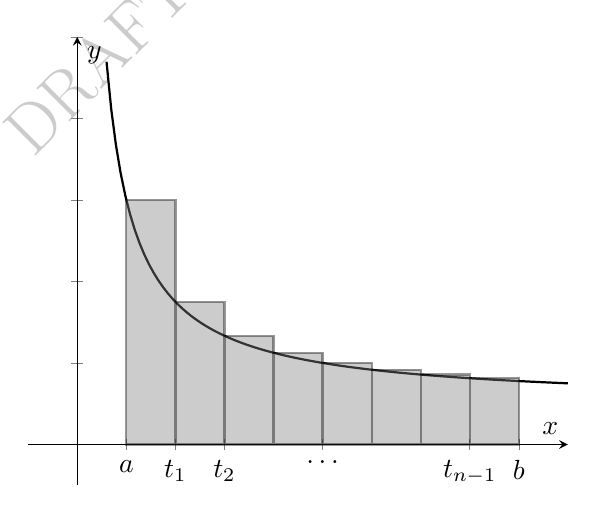
\begin{tikzpicture}
\begin{axis}[xmin=-1, ymin=-1, xmax=10, ymax=10, axis lines=center, xtick={1,2,3,5,8,9}, yticklabels={,,}, xticklabels={$a$,$t_1$,$t_2$, $\ldots$,$t_{n-1}$, $b$}, xlabel=$x$, ylabel=$y$];
\addplot [thick, samples=100, domain=0.5:10, restrict y to domain=0:10]{5*x^(-1)+1};
\addplot [thick,draw=black,fill=gray,opacity=.4, ybar interval, domain=1:9,samples=9]{5*x^(-1)+1};
\end{axis}
\end{tikzpicture}
\end{minipage}
\begin{minipage}{0.45\textwidth}
\subsubsection*{Right-hand Sums}
\begin{equation*}
\int_a^b f(t)\,dt\approx\frac{b-a}{n}(f(t_1)+f(t_2)+\cdots{}+f(t_{n-1})+f(b))
\end{equation*}
\centering
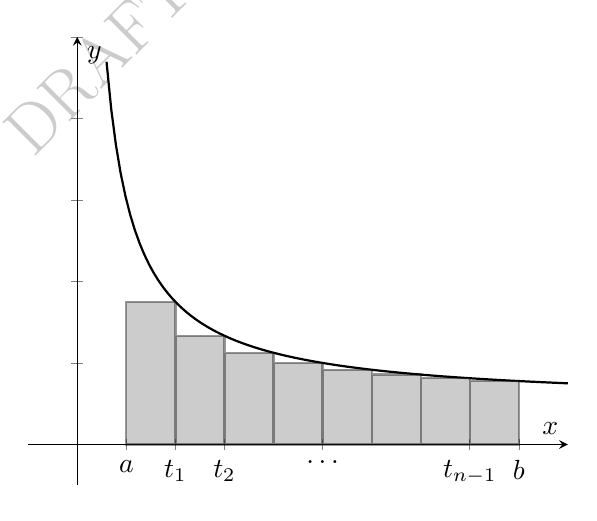
\begin{tikzpicture}
\begin{axis}[xmin=-1, ymin=-1, xmax=10, ymax=10, axis lines=center, xtick={1,2,3,5,8,9}, yticklabels={,,}, xticklabels={$a$,$t_1$,$t_2$, $\ldots$,$t_{n-1}$, $b$}, xlabel=$x$, ylabel=$y$];
\addplot [thick, samples=100, domain=0.5:10, restrict y to domain=0:10]{5*x^(-1)+1};
\addplot [thick,draw=black,fill=gray, opacity=0.4, ybar interval, domain=9:1,samples=9]{5*x^(-1)+1};
\end{axis}
\end{tikzpicture}
\end{minipage}
\begin{verbatim}
\begin{minipage}{0.45\textwidth}
\subsubsection*{Left-hand Sums}
\begin{equation*}
\int_a^b f(t)\,dt\approx{}\frac{b-a}{n}(f(a)+f(t_1)+\cdots{}+f(t_{n-1}))
\end{equation*}
\centering
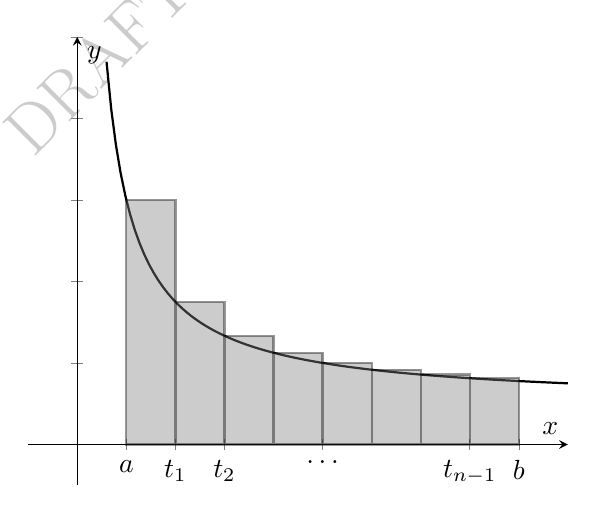
\begin{tikzpicture}
\begin{axis}[xmin=-1, ymin=-1, xmax=10, ymax=10, axis lines=center, xtick={1,2,3,5,8,9}, 
	yticklabels={,,}, xticklabels={$a$,$t_1$,$t_2$, $\ldots$,$t_{n-1}$, $b$}, xlabel=$x$, ylabel=$y$];
\addplot [thick, samples=100, domain=0.5:10, restrict y to domain=0:10]{5*x^(-1)+1};
\addplot [thick,draw=black,fill=gray,opacity=.4, ybar interval, domain=1:9,samples=9]{5*x^(-1)+1};
\end{axis}
\end{tikzpicture}
\end{minipage}
\begin{minipage}{0.45\textwidth}
\subsubsection*{Right-hand Sums}
\begin{equation*}
\int_a^b f(t)\,dt\approx\frac{b-a}{n}(f(t_1)+f(t_2)+\cdots{}+f(t_{n-1})+f(b))
\end{equation*}
\centering
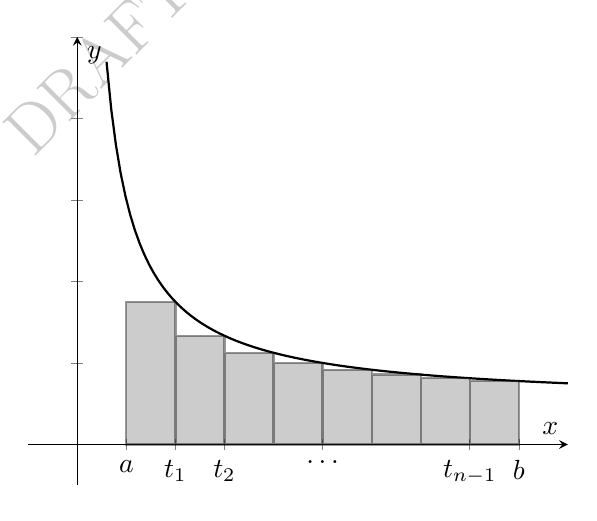
\begin{tikzpicture}
\begin{axis}[xmin=-1, ymin=-1, xmax=10, ymax=10, axis lines=center, xtick={1,2,3,5,8,9}, 
	yticklabels={,,}, xticklabels={$a$,$t_1$,$t_2$, $\ldots$,$t_{n-1}$, $b$}, xlabel=$x$, ylabel=$y$];
\addplot [thick, samples=100, domain=0.5:10, restrict y to domain=0:10]{5*x^(-1)+1};
\addplot [thick,draw=black,fill=gray, opacity=0.4, ybar interval, domain=9:1,samples=9]{5*x^(-1)+1};
\end{axis}
\end{tikzpicture}
\end{minipage}
\end{verbatim}
\subsection{Commutative Diagrams}
Load \verb|\usepackage{tikz-cd}|.  The basic environment is \verb|\begin{tikzcd}...\end{tikzcd}|, the contents are in math mode and should be typed as if in a matrix environment.\\\\
\begin{minipage}{0.45\textwidth}
\centering
\begin{tikzcd}[]
A  \arrow[swap]{rd}{g\circ f} \arrow{r}{f} & B \arrow{d}{g}\\
& C
\end{tikzcd}
\end{minipage}  
\begin{minipage}{0.45\textwidth}
\begin{verbatim}
\begin{tikzcd}[]
A  \arrow[swap]{rd}{g\circ f} \arrow{r}{f} & B \arrow{d}{g}\\
& C
\end{tikzcd}
\end{verbatim}
\end{minipage}\\\\

\section{Graphing}
To produce graphics in \LaTeX~ load these packages in the preamble.  
\begin{verbatim}
\usepackage{tikz}
\usepackage{pgfplots}
    \pgfplotsset{compat=newest}
\end{verbatim}
\subsection{Lines}
\begin{minipage}{0.45\textwidth}
\centering
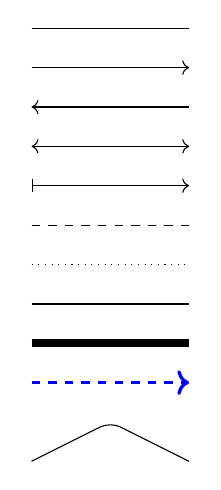
\begin{tikzpicture}
\draw (0,0)--(2,0);
\draw [->] (0,-0.5)--(2,-0.5);
\draw [<-] (0,-1)--(2,-1);
\draw [<->] (0,-1.5)--(2,-1.5);
\draw [|->] (0,-2)--(2,-2);
\draw [dashed] (0,-2.5)--(2,-2.5); 
\draw [dotted] (0,-3)--(2,-3);
\draw [thick] (0,-3.5)--(2,-3.5);
\draw [line width=0.1cm] (0,-4)--(2,-4);
\draw [very thick, dashed, ->,blue](0,-4.5)--(2,-4.5);
\draw [rounded corners] (0,-5.5)--(1,-5)--(2,-5.5);
\end{tikzpicture}
\end{minipage}
\begin{minipage}{0.45\textwidth}
\begin{verbatim}
\centering
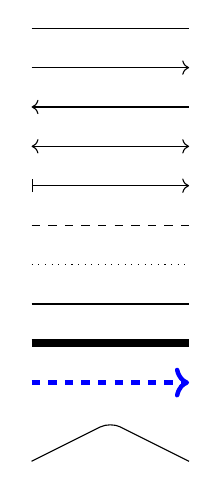
\begin{tikzpicture}
\draw (0,0)--(2,0);
\draw [->] (0,-0.5)--(2,-0.5);
\draw [<-] (0,-1)--(2,-1);
\draw [<->] (0,-1.5)--(2,-1.5);
\draw [|->] (0,-2)--(2,-2);
\draw [dashed] (0,-2.5)--(2,-2.5); 
\draw [dotted] (0,-3)--(2,-3);
\draw [thick] (0,-3.5)--(2,-3.5);
\draw [line width=0.1cm] (0,-4)--(2,-4);
\draw [ultra thick, dashed, ->,blue](0,-4.5)--(2,-4.5);
\draw [rounded corners] (0,-5.5)--(1,-5)--(2,-5.5);
\end{tikzpicture}
\end{verbatim}
\end{minipage}\\\\
In general the command for producing a line is
\begin{verbatim}
\draw [option1,option2,....](a,b)--(c,d)--(e,f);
\end{verbatim}
Note that the coordinates are specified in centimeters.  Some options are
\begin{itemize}
\item[1.]  Arrow decorations.
\item[2.]  Line thickness:  ultra thin, very thin, thin, semithick, thick, very thick, and ultra thick.  Thickness of a line can also be specified by 
\begin{verbatim}
\draw [line width=0.1cm](a,b)--(c,d);
\end{verbatim}
\item[3.]  Colors:  red, green, blue, cyan, magenta, yellow, black, gray, darkgray, lightgray, brown, lime, olive, orange, pink, purple, teal, violet, white.  There is also an option to define custom colors.
\item[4.]  Rounded corners.
\end{itemize}
\subsection{Curves and Shapes}
\begin{center}
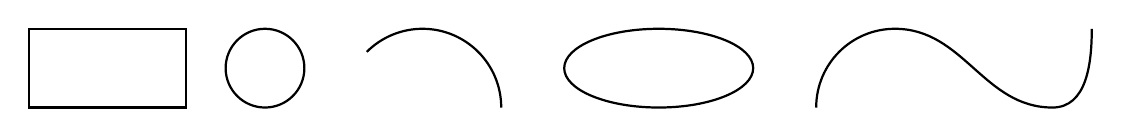
\begin{tikzpicture}
\draw [thick] (0,0) rectangle (2,1);
\draw [thick] (3,0.5) circle [radius=0.5];
\draw [thick] (6,0) arc [radius=1, start angle=0, end angle=135];
\draw [thick] (8,0.5) ellipse [x radius=1.2, y radius =0.5];
\draw [thick] (10,0) to [out=90, in=180] (11,1) to [out=0, in=180] (13,0) to [out=0,in=270] (13.5,1);
\end{tikzpicture}
\end{center}
\begin{verbatim}
\draw [thick] (0,0) rectangle (2,1);
\draw [thick] (3,0.5) circle [radius=0.5];
\draw [thick] (6,0) arc [radius=1, start angle=0, end angle=135];
\draw [thick] (8,0.5) ellipse [x radius=1.2, y radius =0.5];
\draw [thick] (10,0) to [out=90, in=180] (11,1) to [out=0, in=180] (13,0) to [out=0,in=270] (13.5,1);
\end{verbatim}
Note that in the last curve the \verb|out=| specifies the angle that the curve leaves the point, this angle is measured from the tangent line to the curve counterclockwise from a horizontal line.  Likewise the \verb|in=| specifies the angle that the curve approaches the final point. 
\subsection{Axis and Addplot Options}
\subsubsection{Titles and Legends}
A title is added to a plot simply by adding \verb|title=Name| to the axis options.  A legend is also simple to add:
\begin{verbatim}
\begin{axis}[legend entries={a,b,c}, legend style={at={(axis cs:X,Y)}, right}]
\addplot {x};
\addplot {2x};
\addplot {3x};
\end{verbatim}
Note that the legend entries correspond with the order of the addplots, respectively, e.g. $a$ corresponds with the $x$ plot and $b$ corresponds with the $2x$ plot.  The \verb|right| indicates that the legend will be placed to the right of the coordinate $(X,Y)$, the other options are \verb|left|, \verb|above|, \verb|below|, or if left blank then the legend is placed directly on the coordinate.  
\subsubsection{Size}
Normally the default size of a graph is sufficient, however to change the size you can either specify the dimensions absolutely or relatively.  For instance:
\begin{verbatim}
\begin{axis}[width=Xcm, height=Ycm,...]
\end{verbatim}
The above specifies the size of a graph absolutely, whereas the following code uses relative dimensions:
\begin{verbatim}
\begin{axis}[width=0.X\textwidth,...]
\end{verbatim}
You could also use \verb|\begin{axis}[height=0.Y\textheight...]|.  Even though only the width (or height) is specified both axes are scaled similarly.  Another option is to use \verb|scale=X.Y|, this scales the graph by a factor of $X.Y$.
\subsubsection{Axis Tick Marks}
To remove all ticks and tick labels, add \verb|ticks=none| to the \verb|axis| options.  To remove only the tick labels (the ticks themselves will still be present) on either one or both of the axes use \verb|yticklabels={,,}| and/or \verb|xticklabels={,,}|.  To remove both ticks and tick labels from a single axis add \verb|ytick={0}, yticklabels={}|, similar for the $x$-axis.\\\\
For custom tick labels use the \verb|xtick={}| and \verb|xticklabels={}| commands.  For example:
\begin{verbatim}
xtick={1,4,6,9}, xticklabels={$T$, $I$, $A$, $F$}
\end{verbatim}
 places $T$ at $x=1$, $I$ at $x=4$ and so on, similar for the $y$-axis.\\\\
To shift all tick labels use \verb|xticklabel style={xshift=Xcm, yshift=Ycm}|, similar for $y$ ticks.
\subsubsection{Plots with Unbounded Functions}
If a plotted function's range vastly exceeds the \verb|ymax| or \verb|ymin| then a "Dimension too large" error will occur.  This can be avoided by adding \verb|restrict y to domain=X:Y| to the addplot's options.  If a function has a vertical asymptote, sometimes \LaTeX will draw a solid line connecting the function over the asymptote.  This can be avoided by adding \verb|unbounded coords=jump| to the addplot's options.  
\subsection{Plotting Functions}
\begin{minipage}{0.45\textwidth}
\begin{tikzpicture}
\begin{axis}[axis lines=middle,
xmin=-10, xmax=10,
ymin=-10, ymax=10,
xlabel=$x$, ylabel=$y$,
xticklabels={,,},
ytick={1,2,5,9},
yticklabels={$a$,$b$,$c$,$d$}];
\addplot [thick, domain=-5:10, samples=100]{sin(\x r)};
\end{axis}
\end{tikzpicture}
\end{minipage}
\begin{minipage}{0.45\textwidth}
\begin{verbatim}
\begin{tikzpicture}
\begin{axis}[axis lines=middle,
xmin=-10, xmax=10,
ymin=-10, ymax=10,
xlabel=$x$, ylabel=$y$,
xticklabels={,,},
ytick={1,2,5,9},
yticklabels={$a$,$b$,$c$,$d$}];
\addplot [thick, domain=-5:10, samples=100]{sin(\x r)};
\end{axis}
\end{tikzpicture}
\end{verbatim}
\end{minipage}\\
Unfortunately the argument for trigonometric functions is degrees by default, if you want to specify radians you must enclose the argument in double parentheses and use \verb|\x|, in between the right parentheses add \verb|r| (for radian), e.g. \verb|\addplot [samples=100]{cos((2*\x/pi+pi/4) r)};|.  As far as I am aware, you only need to use a forward slash before the variable when changing degrees to radians.  For instance, \verb|cos(x)| or \verb|ln(x)| will graph without error.  The number of samples will determine how smooth the curve is because \LaTeX plots individual points and then connects them to make the curve, generally 100 samples is sufficient.  Note that you do \emph{not} need a forward slash to indicate a function while graphing, unlike when typing text.  Some common functions are
\begin{itemize}
\item[1.]  \verb|factorial(x)|
\item[2.]  \verb|exp(x)| and \verb|ln(x)|
\item[3.]  \verb|log10(x)| and \verb|log2(x)|, note that other bases, e.g. \verb|log5(x)| will \emph{not} work
\item[4.]  \verb|mod(x,y)| = $x$ modulo $y$
\item[5.]  \verb|round(x)|, rounds $x$ to the nearest integer
\item[6.]  \verb|floor(x)| and \verb|ceil(x)|
\item[7.]  \verb|sin(x)|,\verb|cos(x)|,\verb|tan(x)|, note that to graph the other trig. functions you should manually reciprocate these three.
\item[8.]  Euler's number is simply \verb|e| and pi is simply \verb|pi|
\end{itemize}
\subsubsection{Parametric}
You can also graph parametrically.  Note that you can change the default variable, $x$, to whatever variable you choose by defining it in the options.\\
\begin{minipage}{0.45\textwidth}
\centering
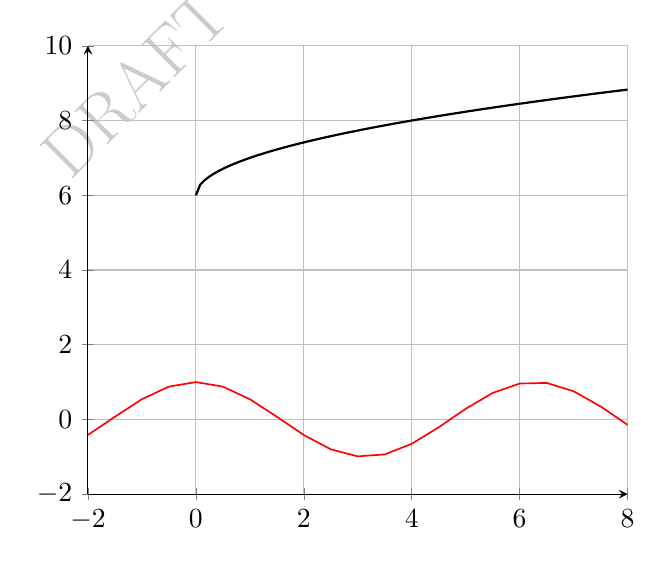
\begin{tikzpicture}
\begin{axis}[axis lines=left,
xmin=-2, xmax=8,
ymin=-2, ymax=10,
grid=both]
\addplot [thick, domain=0:8, samples=100] ({x},{sqrt(x)+6});
\addplot [semithick,red, domain=-2:10, variable=\t] ({t},{cos(\t r)});
\end{axis}
\end{tikzpicture}
\end{minipage}
\hspace{0.5cm}
\begin{minipage}{0.45\textwidth}
\centering
\begin{verbatim}
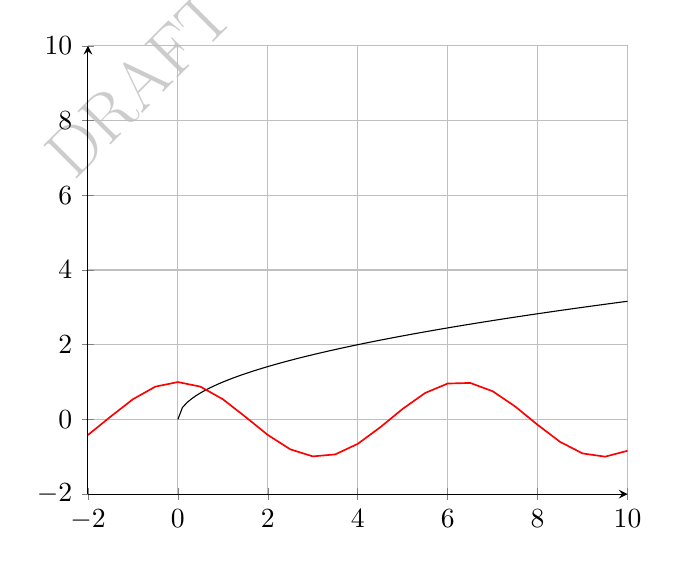
\begin{tikzpicture}
\begin{axis}[axis lines=left,
xmin=-2, xmax=10,
ymin=-2, ymax=10,
grid=both]
\addplot [domain=0:10, samples=100] ({x},{sqrt(x)});
\addplot [semithick,red, domain=-2:10, variable=\t] 
    ({t},{cos(\t r)});
\end{axis}
\end{tikzpicture}
\end{verbatim}
\end{minipage}
\subsubsection{Polar Graphs}
Load \verb|\usepgfplotslibrary{polar}| in the preamble.\\
\begin{minipage}{0.45\textwidth}
\centering
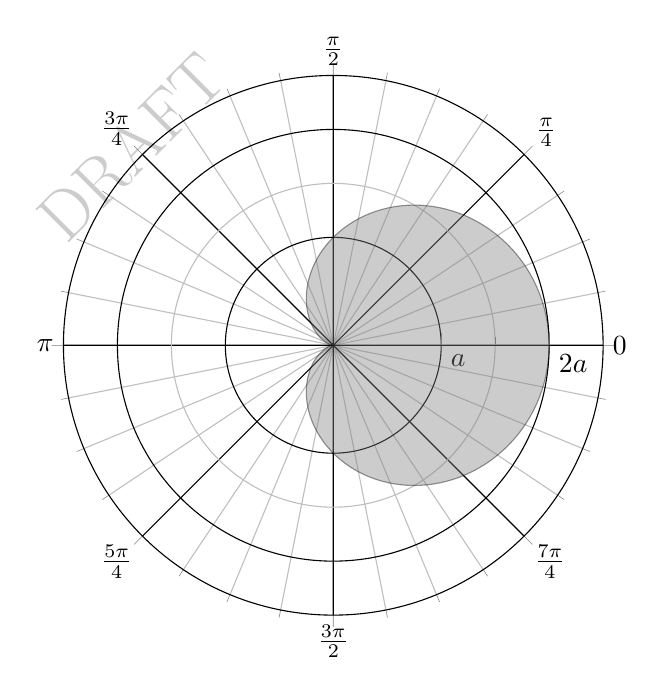
\begin{tikzpicture}
\begin{polaraxis}[domain=0:360,
grid=both, 
minor x tick num=3, 
minor y tick num=1, 
xtick={0,45,90,135,180,225,270,315,360}, 
xticklabels={$0$,$\frac{\pi}{4}$, $\frac{\pi}{2}$,$\frac{3\pi}{4}$,$\pi$,$\frac{5\pi}{4}$,$\frac{3\pi}{2}$,$\frac{7\pi}{4}$}, 
clip=false, 
samples=180, 
major grid style={black},
yticklabel style={anchor=north west},
ymax=5,
ytick={2,4},
yticklabels={$a$,$2a$}];
\addplot[domain=0:360,fill=gray, opacity=0.4]{2+2*cos(x)};
\end{polaraxis}
\end{tikzpicture}
\end{minipage}
\begin{minipage}{0.45\textwidth}
\begin{verbatim}
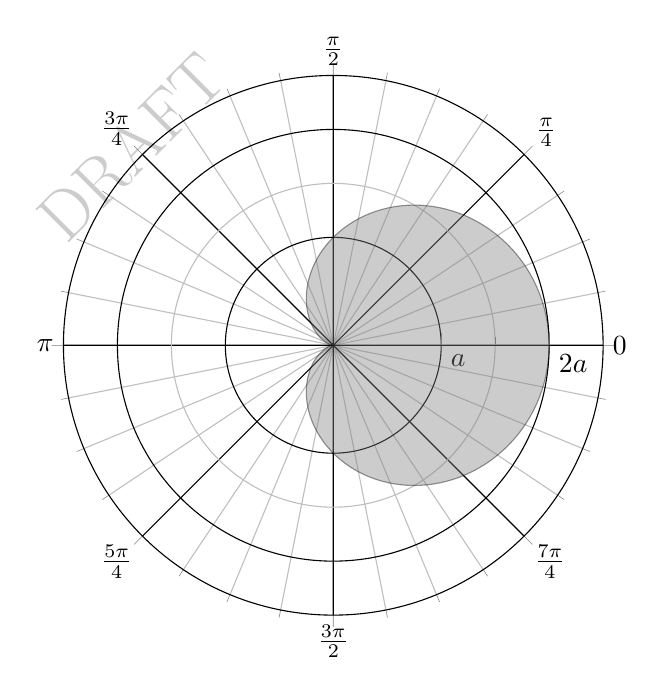
\begin{tikzpicture}
\begin{polaraxis}[domain=0:360,
grid=both, 
minor x tick num=3, 
minor y tick num=1, 
xtick={0,45,90,135,180,225,270,315,360}, 
xticklabels={$0$,$\frac{\pi}{4}$, 
    $\frac{\pi}{2}$,$\frac{3\pi}
    {4}$,$\pi$,$\frac{5\pi}{4}$,
    $\frac{3\pi}{2}$,$\frac{7\pi}{4}$}, 
clip=false, 
samples=180, 
major grid style={black},
yticklabel style={anchor=north west},
ymax=5,
ytick={2,4},
yticklabels={$a$,$2a$}];
\addplot[domain=0:360,fill=gray, opacity=0.4]{2+2*cos(x)};
\end{polaraxis}
\end{tikzpicture}
\end{verbatim}
\end{minipage}\\
Note that $x$ represents the azimuthal angle, normally denoted $\theta$, and $y$ is the radius.  In addition to a polar axis there is also semilogxaxis, semilogyaxis, and loglogaxis.  
\subsection{Decorations}
Load \verb|\usetikzlibrary{decorations.markings}| in the preamble.
\subsubsection{Adding Arrow Tips to Plots}
\begin{minipage}{0.65\textwidth}
\begin{verbatim}
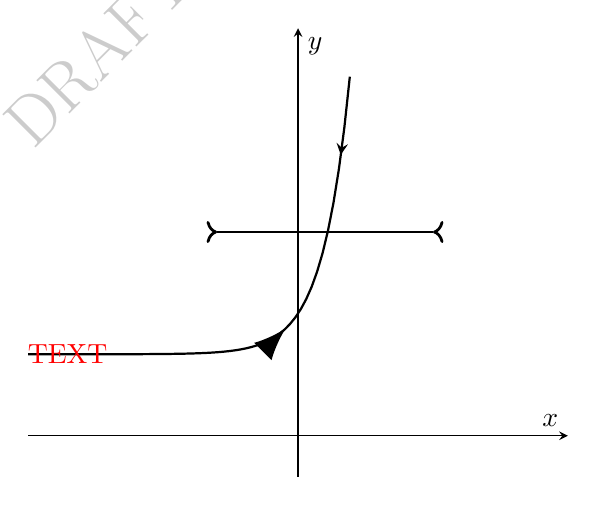
\begin{tikzpicture}
\begin{axis}[xlabel=$x$, ylabel=$y$, xmin=-10, 
	ymin=-1, xmax=10, ymax=10, axis lines=middle, ticks=none]
\addplot [thick,variable=\t, samples=100, domain=-10:10, 
	restrict y to domain=-1:10,
	postaction={decorate}, 
	decoration={markings, 
	mark= at position 0.5cm with {\node[red]{TEXT};},
	mark= at position 0.5 with {\arrow[line width=3pt]{latex};},
	mark= at position -1cm with {\arrowreversed{stealth};}}
	]
	({t}, {e^t+2});
	\draw[thick,postaction={decorate},decoration={markings,
	mark= at position 0 with {\arrow[line width=1 pt]{>};},
	mark= at position 1 with {\arrowreversed[line width=1 pt]{>};}}
	]
	(axis cs:-3,5)--(axis cs:5,5);
\end{axis}
\end{tikzpicture}
\end{verbatim}
\end{minipage}
\begin{minipage}{0.3\textwidth}
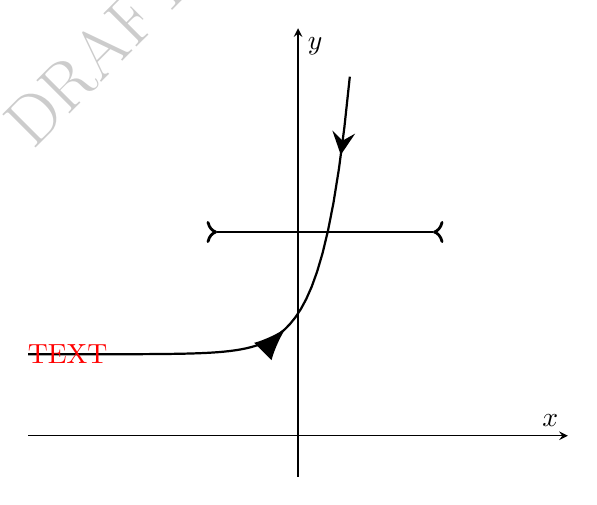
\begin{tikzpicture}
\begin{axis}[xlabel=$x$, ylabel=$y$, xmin=-10, ymin=-1, xmax=10, ymax=10, axis lines=middle, ticks=none]
\addplot [thick,variable=\t, samples=100, domain=-10:10, restrict y to domain=-1:10,
	postaction={decorate}, 
	decoration={markings, 
	mark= at position 0.5cm with {\node[red]{TEXT};},
	mark= at position 0.5 with {\arrow[line width=3pt]{latex};},
	mark= at position -1cm with {\arrowreversed[scale=2]{stealth};}}
	]
	({t}, {e^t+2});
	\draw[thick,postaction={decorate},decoration={markings,
	mark= at position 0 with {\arrow[line width=1 pt]{>};},
	mark= at position 1 with {\arrowreversed[line width=1 pt]{>};}}
	]
	(axis cs:-3,5)--(axis cs:5,5);
\end{axis}
\end{tikzpicture}
\end{minipage}\\\\
The \verb|postaction={decorate}| command tells \LaTeX that some kind of decoration will take place \emph{after} the main action has taken place, e.g. after the function has been plotted.  \verb|decoration={markings, mark=...}| indicates the type of decoration is markings and the \verb|mark=...| is the beginning of the first decoration.  You may use any number of decorations.  Note the semi-colons following \emph{each} mark description.  Also note that when specifying different arrow tip types you do not need to use a hyphen, e.g. \verb|{>}| not \verb|{->}|.  Lastly note that the tip of arrow is placed on the curve, this may cause the back end of the arrow to lay off the curve if the arrow is made larger, as in the example above.
\subsubsection{Arrow Tip Types and Sizes}
Refer to Table \ref{tb:arrow} (on page \pageref{tb:arrow}).  Other styles not included in the table are \verb|To|, \verb|Computer Modern Rightarrow|, \verb|Diamond|, \verb|Circle|, \verb|Kite|, \verb|Rectangle|, \verb|Square|.  
\begin{table}[b!]
\centering
\renewcommand{\arraystretch}{1.5}
\begin{tabular}{lc}
\hline
Code & Example \\
\hline
\verb|\draw [-stealth] (-1,0)--(0,0);| & \begin{tikzpicture}
\draw [-stealth] (-1,0)--(0,0);
\end{tikzpicture} \\
\verb|\draw [-Stealth] (-1,0)--(0,0);| & \begin{tikzpicture}
\draw [-Stealth] (-1,0)--(0,0);
\end{tikzpicture}\\
\verb|\draw [->] (-1,0)--(0,0);| & \begin{tikzpicture}
\draw [->] (-1,0)--(0,0);
\end{tikzpicture} \\
\verb|\draw [-latex] (-1,0)--(0,0);| & \begin{tikzpicture}
\draw [-latex] (-1,0)--(0,0);
\end{tikzpicture} \\
\verb|\draw [-{Latex[length=3mm, width=3mm]}] (-1,0)--(0,0);| & 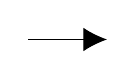
\begin{tikzpicture}
\draw [-{Latex[length=3mm, width=3mm]}](-1,0)--(0,0);
\end{tikzpicture} \\
\verb|\draw [-.>.>.>.>] (-1,0)--(0,0);| & 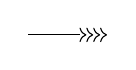
\begin{tikzpicture}
\draw [-.>.>.>.>] (-1,0)--(0,0);
\end{tikzpicture}\\
\verb|\draw [-{Triangle[scale=2,open]}] (-1,0)--(0,0);| & \begin{tikzpicture}
\draw [-{Triangle[scale=2,open]}] (-1,0)--(0,0);
\end{tikzpicture}\\
\verb|\draw [-Parenthesis] (-1,0)--(0,0);| & \begin{tikzpicture}
\draw [-Parenthesis] (-1,0)--(0,0);
\end{tikzpicture}\\
\verb|\draw [-Bar] (-1,0)--(0,0);| & \begin{tikzpicture}
\draw [-Bar] (-1,0)--(0,0);
\end{tikzpicture}\\
\verb|\draw [-Bracket] (-1,0)--(0,0);| & \begin{tikzpicture}
\draw [-Bracket] (-1,0)--(0,0);
\end{tikzpicture}\\
\hline
\end{tabular}
\caption{Arrow Styles}\label{tb:arrow}
\end{table}
\subsection{Shading Areas}
\subsubsection{Simple Regions}
\begin{center}
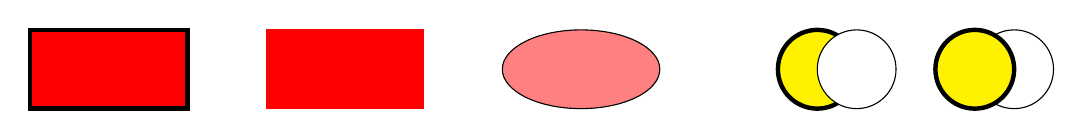
\begin{tikzpicture}
\draw [fill=red,ultra thick] (0,0) rectangle (2,1);
\draw [fill=red,red] (3,0) rectangle (5,1);
\draw [fill=red!50] (7,0.5) ellipse [x radius=1, y radius=0.5];
\draw [fill=yellow,ultra thick] (10,0.5) circle [radius=0.5];
\draw [fill=white] (10.5,0.5) circle [radius=0.5];
\draw [fill=white] (12.5,0.5) circle [radius=0.5];
\draw [fill=yellow,ultra thick] (12,0.5) circle [radius=0.5];
\end{tikzpicture}
\end{center}
\begin{verbatim}
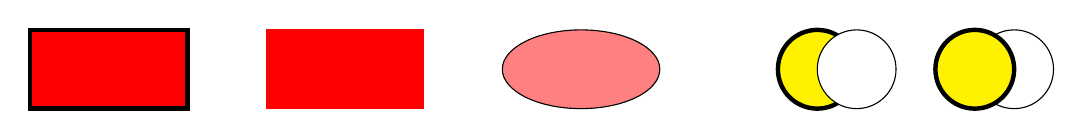
\begin{tikzpicture}
\draw [fill=red,ultra thick] (0,0) rectangle (2,1);
\draw [fill=red,red] (3,0) rectangle (5,1);
\draw [fill=red!50] (7,0.5) ellipse [x radius=1, y radius=0.5];
\draw [fill=yellow,ultra thick] (10,0.5) circle [radius=0.5];
\draw [fill=white] (10.5,0.5) circle [radius=0.5];
\draw [fill=white] (12.5,0.5) circle [radius=0.5];
\draw [fill=yellow,ultra thick] (12,0.5) circle [radius=0.5];
\end{tikzpicture}
\end{verbatim}
Note that \verb|!50| indicates that the lightness (note this is not opacity, the object will still be opaque) of the color is 50\%.  By default \LaTeX will draw a black line around your shape, if you want to change the color of the line simply specify a color, as in the second rectangle above.  Notice that in the overlaying circles it is the \emph{order} in which they are drawn that determines which sits on top of which. 
\subsubsection{Intersections of Simple Regions}
Similar to newspaper clippings you can clip regions and keep just the clippings.  The \verb|\clip| command is followed by whatever shape you wish to clip, all subsequent shapes or fillings in the drawing are drawn if and only if they fall inside the clipping region.  If a clip command is enclosed in a scope environment then it only affects what is drawn/filled in that particular environment.  In the case of multiple clip commands, the intersection of all the regions is used.\\\\
\begin{minipage}{0.45\textwidth}
\centering
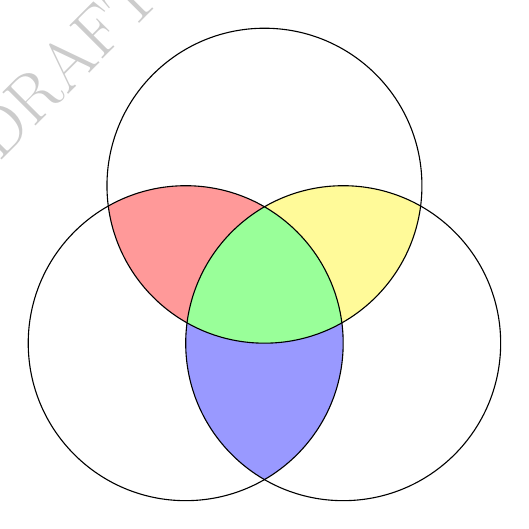
\begin{tikzpicture}
\begin{scope}
\clip (0,0) circle (2);
\fill[red!40] (1,2) circle (2);
\end{scope}
\begin{scope}
\clip(2,0) circle (2);
\fill[yellow!40] (1,2) circle (2);
\end{scope}
\begin{scope}
\clip (0,0) circle (2);
\fill[blue!40] (2,0) circle (2);
\end{scope}
\begin{scope}
\clip (0,0) circle (2);
\clip (2,0) circle (2);
\fill[green!40] (1,2) circle (2);
\end{scope}
\draw (0,0) circle (2);
\draw (2,0) circle (2);
\draw (1,2) circle (2);
\end{tikzpicture}
\end{minipage}  
\begin{minipage}{0.45\textwidth}
\begin{verbatim}
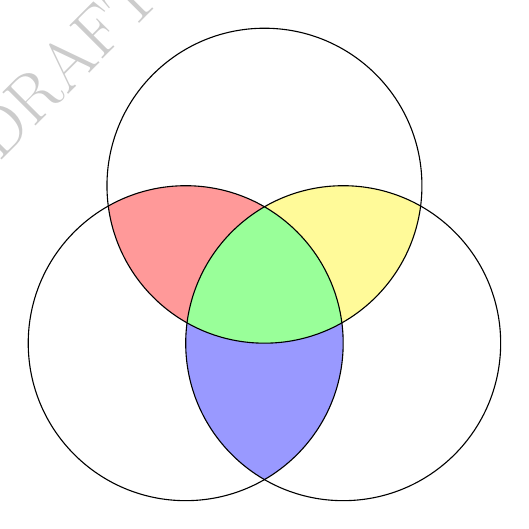
\begin{tikzpicture}
\begin{scope}
	\clip (0,0) circle (2);
	\fill[red!40] (1,2) circle (2);
\end{scope}
\begin{scope}
	\clip(2,0) circle (2);
	\fill[yellow!40] (1,2) circle (2);
\end{scope}
\begin{scope}
	\clip (0,0) circle (2);
	\fill[blue!40] (2,0) circle (2);
\end{scope}
\begin{scope}
	\clip (0,0) circle (2);
	\clip (2,0) circle (2);
	\fill[green!40] (1,2) circle (2);
\end{scope}
\draw (0,0) circle (2);
\draw (2,0) circle (2);
\draw (1,2) circle (2);
\end{tikzpicture}
\end{verbatim}
\end{minipage}
\subsubsection{Even Odd Rule}
The even odd rule is an algorithm for determining which points lie inside or outside a polygon.  In each region of the polygon choose a point and draw a ray, then count the number of times this ray intersects the polygon.  If that number is odd the point (and hence that whole region) is said to be inside the polygon.  If the number is even the point/region is considered to be outside the polygon.  When the even odd rule is used to shade areas \LaTeX will shade areas that are inside the polygon and not shade areas that are outside.  For example,
\begin{center}
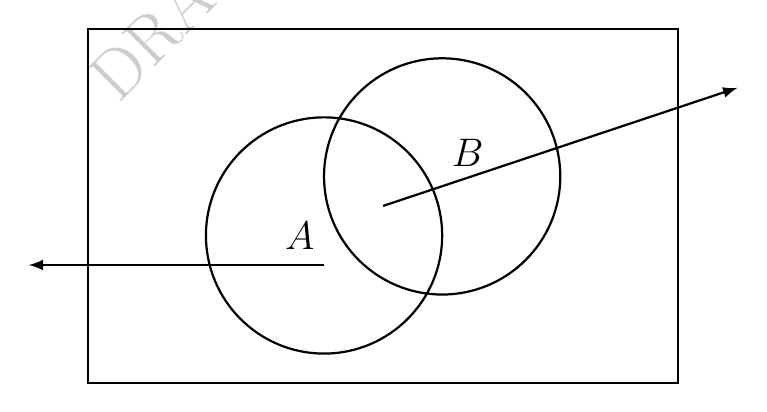
\begin{tikzpicture}[scale=0.75]
\draw[thick] (-5,-3) rectangle (5,3);
\draw [thick] (-1,-0.5) circle (2);
\draw [thick] (1,0.5) circle (2);
\draw [thick,-latex](0,0)--(6,2);
\draw [thick,-latex](-1,-1)--(-6,-1);
\node [left] at (-1,-0.5)(){\Large$A$};
\node [above right] at (1,0.5)(){\Large$B$};
\end{tikzpicture}
\end{center}
Notice that the ray from region $A$ intersects the circle/rectangle shape twice and is thus considered inside.  The ray from $A\cap{}B$ however intersects the shape three times and is considered outside.  Using this we can shade the region $A\cap{}B^C$:\\\\
\begin{minipage}{0.45\textwidth}
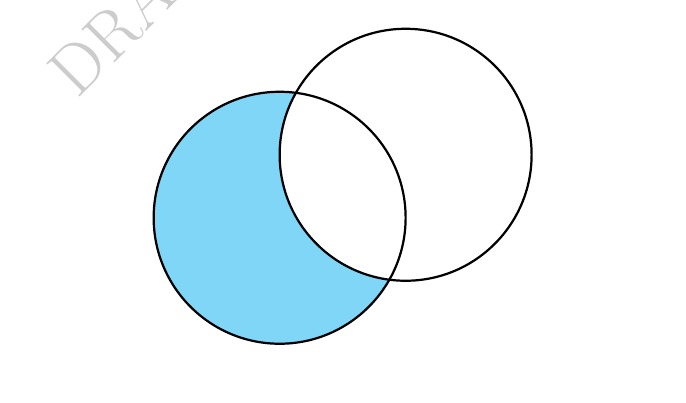
\begin{tikzpicture}[scale=0.8]
\begin{scope}
\clip (1,0.5) circle (2) (-5,-3) rectangle (5,2);
\fill [cyan!50] (-1,-0.5) circle (2);
\end{scope}
\draw [thick](1,0.5) circle (2);
\draw [thick](-1,-0.5) circle (2);
\end{tikzpicture}
\end{minipage}
\begin{minipage}{0.45\textwidth}
\begin{verbatim}
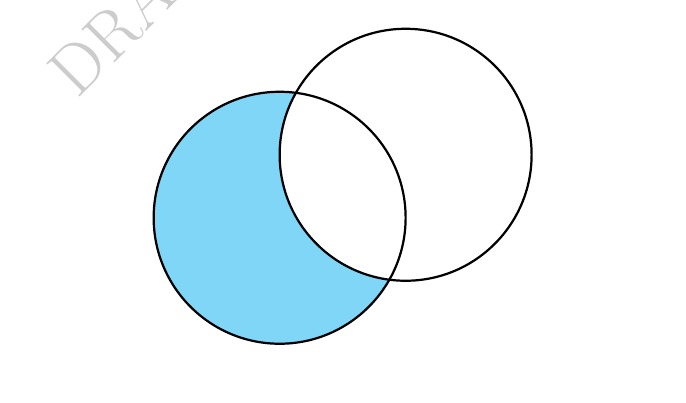
\begin{tikzpicture}[scale=0.8]
\begin{scope}
\clip (1,0.5) circle (2) (-5,-3) rectangle (5,2);
\fill [cyan!50] (-1,-0.5) circle (2);
\end{scope}
\draw [thick](1,0.5) circle (2);
\draw [thick](-1,-0.5) circle (2);
\end{tikzpicture}
\end{verbatim}
\end{minipage}\\\\
Note that the circle and the rectangle are included on the same in the clip command, this is because you want to consider them together as a single shape.
\subsubsection{Arbitrary Areas}
You must load \verb|\usepgfplotslibrary{fillbetween}| in the preamble to shade areas between functions. 
\begin{minipage}{0.45\textwidth}
\vspace{10pt}
\hspace{-1.5cm}
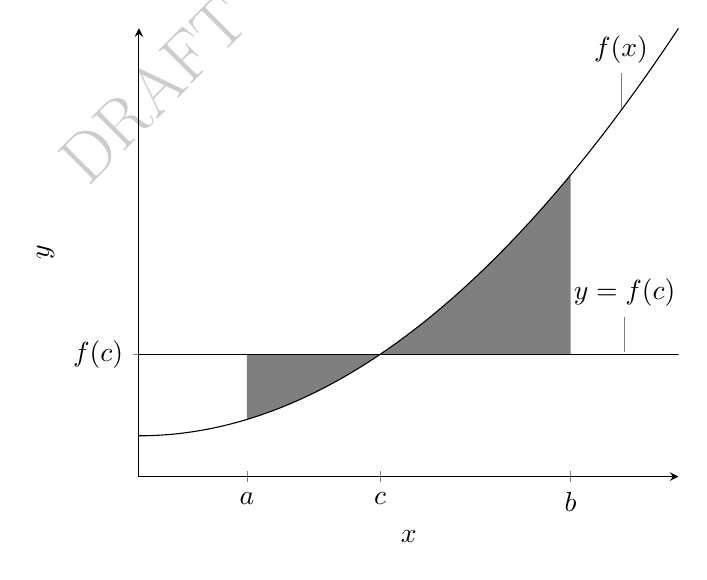
\begin{tikzpicture}
\begin{axis}[xmin=0, xmax=10, 
ymin=-10, ymax=100, 
axis lines=left, 
xlabel=$x$, ylabel=$y$, 
xtick={2,4.47,8}, ytick={20},
yticklabels={$f(c)$}, xticklabels={$a$,$c$,$b$}]
\addplot [name path=f, domain=0:10, samples=100] {x^2}node [pos=0.8, pin={$f(x)$}, inner sep =0 pt]{};
\addplot [name path=c, domain=0:10, samples=100] {20}node [pos=0.9, pin={$y=f(c)$}, inner sep=0 pt]{};
\addplot [thick, color=black, fill=black, fill opacity=0.5] fill between[of=f and c, soft clip={domain=2:8}];
\end{axis}
\end{tikzpicture}
\end{minipage}
\begin{minipage}{0.45\textwidth}
\begin{verbatim}
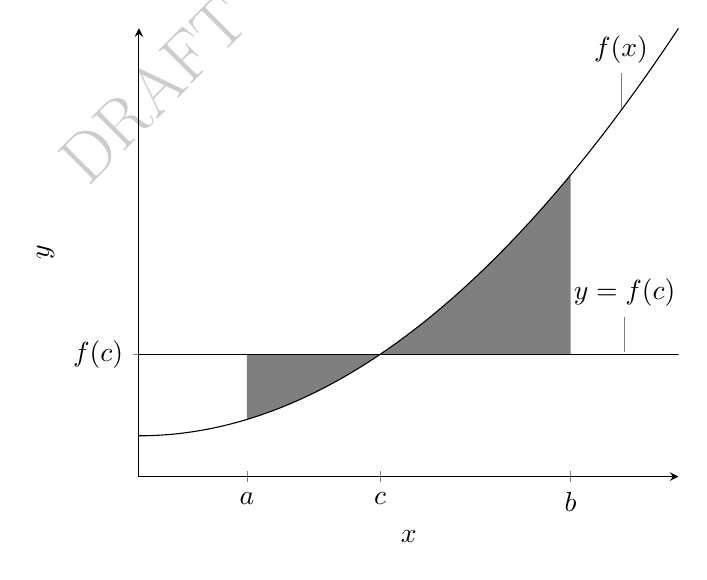
\begin{tikzpicture}
\begin{axis}[xmin=0, xmax=10, 
ymin=-10, ymax=100, 
axis lines=left, 
xlabel=$x$, ylabel=$y$, 
xtick={2,4.47,8}, ytick={20},
yticklabels={$f(c)$}, xticklabels={$a$,$c$,$b$}]
\addplot [name path=f, domain=0:10, samples=100] {x^2}
    node [pos=0.8, pin={$f(x)$}, inner sep =0 pt]{};
\addplot [name path=c, domain=0:10, samples=100] {20}
    node [pos=0.9, pin={$y=f(c)$}, inner sep=0 pt]{};
\addplot [thick, color=black, fill=black, fill opacity=0.5] 
    fill between[of=f and c, soft clip={domain=2:8}];
\end{axis}
\end{tikzpicture}
\end{verbatim}
\end{minipage}\\
Note that the \verb|node| is used to labeling the function, \verb|pos| indicates how far along the curve the label should be placed, \verb|pin| declares the actual label, and \verb|inner sep| is used to offset the label from the function.  There is a slightly more advanced option for when there are multiple regions to be shaded.\\
\begin{minipage}{0.45\textwidth}
\centering
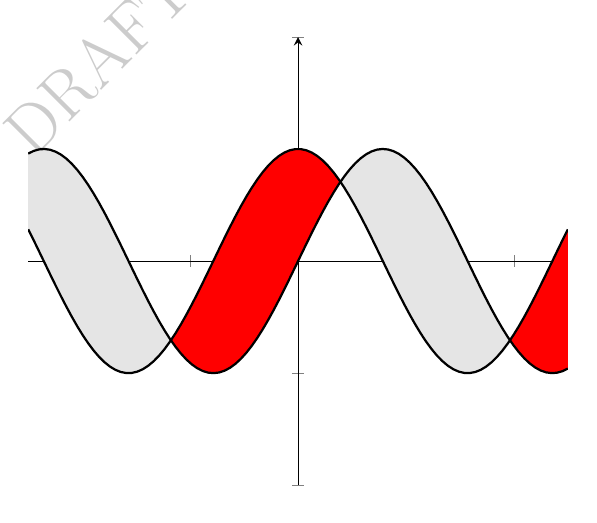
\begin{tikzpicture}
\begin{axis}[axis lines=middle,
xmin=-5, xmax=5,
ymin=-2, ymax=2,
xticklabels={,,}, yticklabels={,,}]
\addplot [name path=c,thick, domain=-5:5, samples=100] {cos(\x r)};
\addplot [name path=s,thick, domain=-5:5, samples=100] {sin(\x r)};
\addplot fill between [of=c and s, split, 
    every even segment/.style={gray!20}, 
    every odd segment/.style={red}];
\end{axis}
\end{tikzpicture}
\end{minipage}
\begin{minipage}{0.45\textwidth}
\begin{verbatim}
\begin{axis}[axis lines=middle,
xmin=-5, xmax=5,
ymin=-2, ymax=2,
xticklabels={,,}, yticklabels={,,}]
\addplot [name path=c,thick, domain=-5:5, samples=100] 
    {cos(\x r)};
\addplot [name path=s,thick, domain=-5:5, samples=100] 
    {sin(\x r)};
\addplot fill between [of=c and s, split, 
    every even segment/.style={gray!20}, 
    every odd segment/.style={red}];
\end{axis}
\end{tikzpicture}
\end{verbatim}
\end{minipage}
\subsection{Scatterplots}
\begin{minipage}{0.45\textwidth}
\hspace{-1cm}
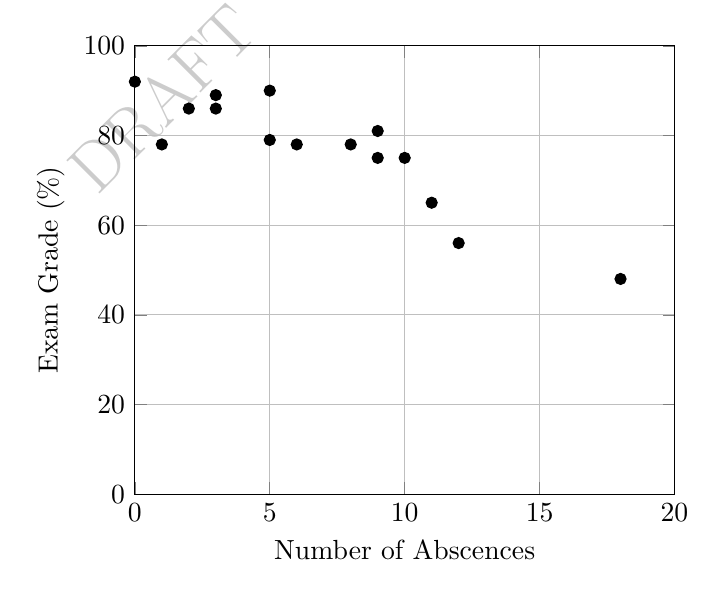
\begin{tikzpicture}
\begin{axis}[xlabel=Number of Abscences, 
xmin=0, xmax=20, 
ylabel=Exam Grade (\%), 
ymin=0, ymax=100, 
grid=both]
\addplot[mark=*, only marks] coordinates {
(5,79)
(6,78)
(2,86)
(12,56)
(9,75)
(5,90)
(8,78)
(18,48)
(0,92)
(1,78)
(9,81)
(3,86)
(10,75)
(3,89)
(11,65)
};
\end{axis}
\end{tikzpicture}
\end{minipage}
\begin{minipage}{0.45\textwidth}
\begin{verbatim}
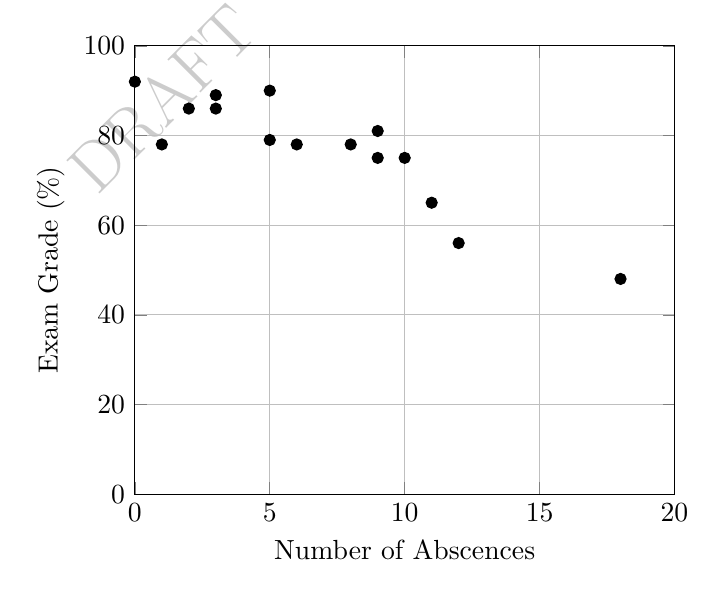
\begin{tikzpicture}
\begin{axis}[xlabel=Number of Abscences, 
xmin=0, xmax=20, 
ylabel=Exam Grade (\%), 
ymin=0, ymax=100, 
grid=both]
\addplot[mark=*, only marks] coordinates {
(5,79)
(6,78)
(2,86)
(12,56)
(9,75)
(5,90)
(8,78)
(18,48)
(0,92)
(1,78)
(9,81)
(3,86)
(10,75)
(3,89)
(11,65)
};
\end{axis}
\end{tikzpicture}
\end{verbatim}
\end{minipage}\\
Other \verb|mark| types are \verb|x|, \verb|+|, |, \verb|o|, asterisk, star, 10-pointed star, oplus, oplus*, otimes, otimes*, square, square*, triangle, triangle*, diamond, halfdiamond*, halfsquare*, right*, left*, Mercedes star, Mercedes star flipped, halfcircle, halfcircle*, pentagon, pentagon*.  
\subsection{Nodes}
Nodes are useful for labeling drawings and graphs.  As will be seen nodes can be labeled which is very useful and expeditious later when drawing lines between nodes or referencing positions.  
\subsubsection{Absolute Position}
The general notation is
\begin{verbatim}
\node [option1, option2,....] at (a,b)(label){Text};
\end{verbatim}
\begin{minipage}{0.45\textwidth}
\centering
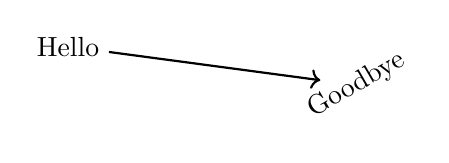
\begin{tikzpicture}
\node [above left] at (0,0)(1) {Hello};
\node [below, rotate=30] at (3,0)(2) {Goodbye};
\draw [->, thick](1)--(2);
\end{tikzpicture}  
\end{minipage}
\begin{minipage}{0.45\textwidth}
\begin{verbatim}
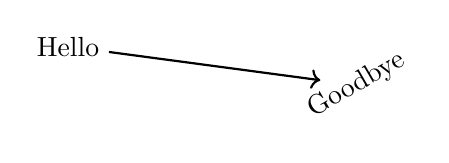
\begin{tikzpicture}
\node [above left] at (0,0)(1) {Hello};
\node [below, rotate=30] at (3,0)(2) {Goodbye};
\draw [->, thick](1)--(2);
\end{tikzpicture}
\end{verbatim}
\end{minipage}\\
Note that the position options are \verb|above|, \verb|above left|, \verb|above right|, \verb|right|, \verb|left|, \verb|below left|, \verb|below right|.  Also notice that you can rotate the node text, again the angle is measured counterclockwise from a horizontal line.  
\subsubsection{Relative Position}
Load \verb|\usetikzlibrary{positioning}| in the preamble.\\
\begin{minipage}{0.45\textwidth}
\centering
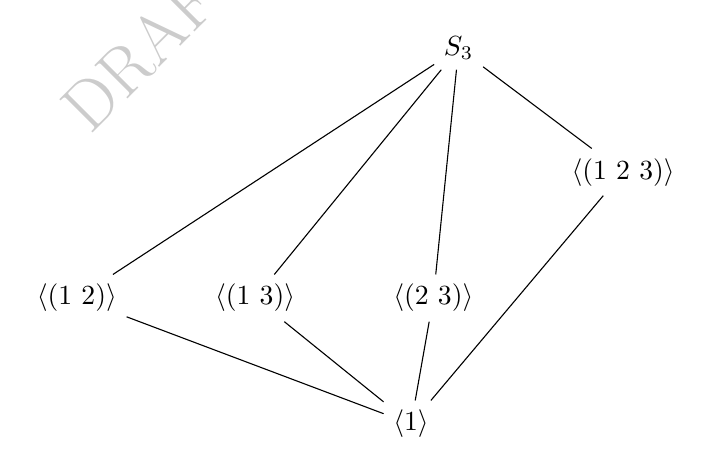
\begin{tikzpicture}
\node at(0,0)(1) {$S_3$};
\node [below right=of 1](2) {$\langle(1~2~3)\rangle$};
\node [below left=of 2](3) {$\langle(2~3)\rangle$};
\node [left=of 3](4) {$\langle(1~3)\rangle$};
\node [left=of 4](5) {$\langle(1~2)\rangle$};
\node [below right=of 4](6) {$\langle{}1\rangle$};
\draw (1)--(2);
\draw (2)--(6);
\draw (1)--(3);
\draw (1)--(4);
\draw (1)--(5);
\draw (3)--(6);
\draw (4)--(6);
\draw (5)--(6);
\end{tikzpicture}
\end{minipage}
\hspace{1cm}
\begin{minipage}{0.45\textwidth}
\begin{verbatim}
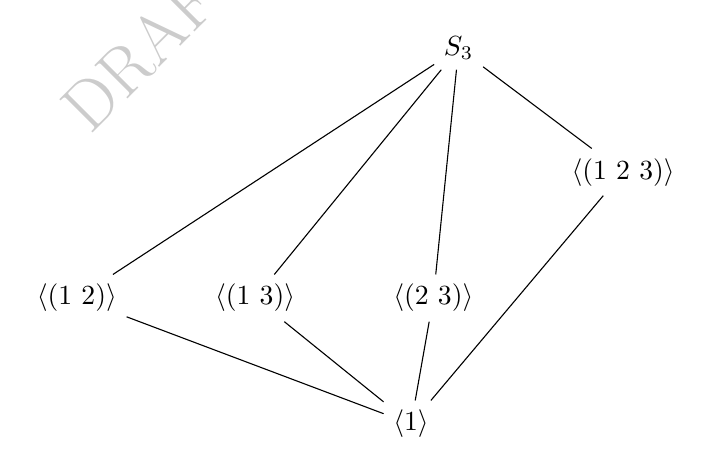
\begin{tikzpicture}
\node at(0,0)(1) {$S_3$};
\node [below right=of 1](2) {$\langle(1~2~3)\rangle$};
\node [below left=of 2](3) {$\langle(2~3)\rangle$};
\node [left=of 3](4) {$\langle(1~3)\rangle$};
\node [left=of 4](5) {$\langle(1~2)\rangle$};
\node [below right=of 4](6) {$\langle{}1\rangle$};
\draw (1)--(2);
\draw (2)--(6);
\draw (1)--(3);
\draw (1)--(4);
\draw (1)--(5);
\draw (3)--(6);
\draw (4)--(6);
\draw (5)--(6);
\end{tikzpicture}
\end{verbatim}
\end{minipage}
\subsubsection{Curved Arrows}
\begin{minipage}{0.45\textwidth}
\centering
\begin{tikzpicture}
\node at (0,0)(1){$A$};
\node [left=of 1](2) {$B$};
\node [below right=of 1](3) {$C$};
\draw [style=dashed,->] (2) to[out=0, in=90] (1);
\draw [->] (1) to[out=45,in=90] (3);
\draw [->] (3) to[out=180,in=-90](1);
\end{tikzpicture}
\end{minipage}
\begin{minipage}{0.45\textwidth}
\begin{verbatim}
\begin{tikzpicture}
\node at (0,0)(1){$A$};
\node [left=of 1](2) {$B$};
\node [below right=of 1](3) {$C$};
\draw [style=dashed,->] (2) to[out=0, in=90] (1);
\draw [->] (1) to[out=45,in=90] (3);
\draw [->] (3) to[out=180,in=-90](1);
\end{tikzpicture}
\end{verbatim}
\end{minipage}
\subsubsection{Typing Multiple Lines in Nodes}
\begin{minipage}{0.45\textwidth}
\centering
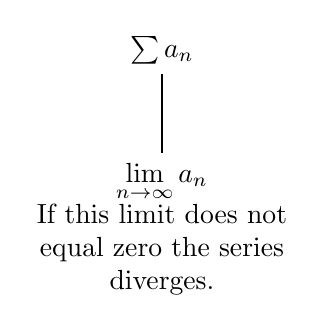
\begin{tikzpicture}
\node at (0,0)(1) {$\sum a_n$};
\node [align=center, below=of 1](2) {$\displaystyle \lim_{n\to\infty}a_n$\\
If this limit does not\\
equal zero the series\\
diverges.};
\draw (1)--(2);
\end{tikzpicture}
\end{minipage}
\begin{minipage}{0.45\textwidth}
\begin{verbatim}
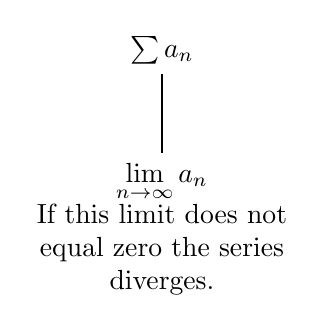
\begin{tikzpicture}
\node at (0,0)(1) {$\sum a_n$};
\node [align=center, below=of 1](2) 
    {$\displaystyle \lim_{n\to\infty}a_n$\\
    If this limit does not\\
    equal zero the series\\
    diverges.};
\draw (1)--(2);
\end{tikzpicture}
\end{verbatim}
\end{minipage}\\\\
The \verb|align| command allows you to type multiple lines in a node, otherwise all the text will be on the same line.  Besides centering you can also use \verb|align=left| or \verb|align=right|.
\subsubsection{Nodes in Graphs}
\begin{minipage}{0.45\textwidth}
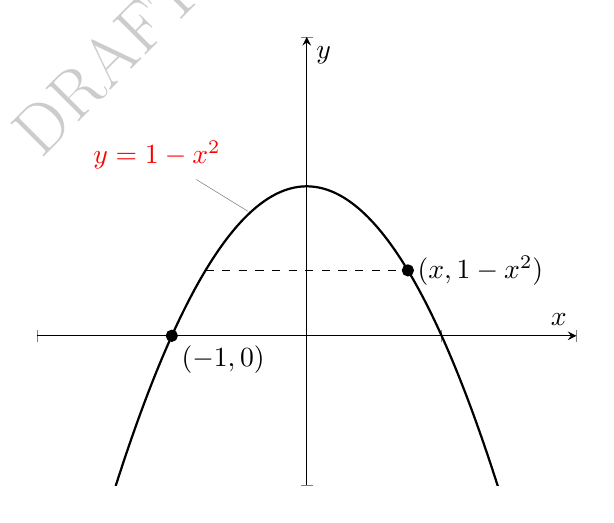
\begin{tikzpicture}
\begin{axis}[xmin=-2, xmax=2, 
ymin=-1, ymax=2, 
yticklabels={,,}, xticklabels={,,}, 
axis lines=middle, 
xlabel=$x$, ylabel=$y$,]
\addplot [thick, domain=-2:2, samples=200] {1-x^2} node [rotate=30,pos=0.45, pin={[red]$y=1-x^2$}, inner sep=0 pt]{};
\draw [style=dashed](axis cs:-0.75,0.4375) --(axis cs:0.75,0.4375) node[right]{$(x,1-x^2)$};
\node [anchor=north west] at (axis cs:-1,0)(){$(-1,0)$};
\addplot [mark=*, only marks]coordinates {(0.75,0.4375)(-1,0)};
\end{axis}
\end{tikzpicture}
\end{minipage}
\begin{minipage}{0.45\textwidth}
\begin{verbatim}
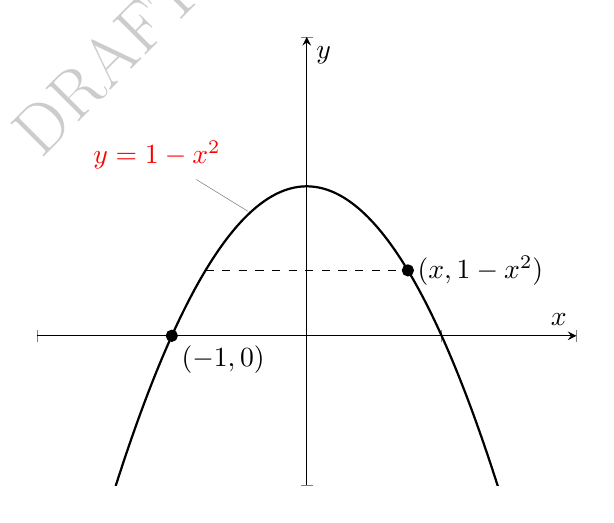
\begin{tikzpicture}
\begin{axis}[xmin=-2, xmax=2, 
ymin=-1, ymax=2, 
yticklabels={,,}, xticklabels={,,}, 
axis lines=middle, 
xlabel=$x$, ylabel=$y$,]
\addplot [thick, domain=-2:2, samples=200] {1-x^2} 
    node [rotate=30,pos=0.45, pin={[red]$y=1-x^2$}, 
    inner sep=0 pt]{};
\draw [style=dashed](axis cs:-0.75,0.4375) 
    --(axis cs:0.75,0.4375) node[right]{$(x,1-x^2)$};
\node [anchor=north west] at (axis cs:-1,0)(){$(-1,0)$};
\addplot [mark=*, only marks]
    coordinates {(0.75,0.4375)(-1,0)};
\end{axis}
\end{tikzpicture}
\end{verbatim}
\end{minipage}\\
There are several things to note.  First, the exact same syntax for nodes can be used in graphs.  However, \LaTeX will, by default, \emph{not} reference the origin of the axis for positions unless \verb|axis cs:| is specified before the coordinates.  The position of the last node is specified by the \verb|anchor| system, as far as I am aware there is no difference between this and just specifying \verb|left| or \verb|right|.  The issue with the \verb|anchor| system is that the directions are reversed.  For instance, if you want a label to appear above something you have to specify \verb|anchor=south|, instead of the more intuitive \verb|north|.  Lastly note that the label for the function can be rotated and also note the position for the options for the actual text of the label is located inside the \verb|pin| brackets.
\subsection{Flowcharts}  
\subsection{3-Dimensional Plots}
\LaTeX is not meant to graph complex visuals and it will take a fair amount of time for a 3-dimensional plot to process.  You can graph using either cartesian equations or parametrically.  Generally parametrically is the better option.  
\subsubsection{Parametric}
\begin{minipage}{0.45\textwidth}
\centering
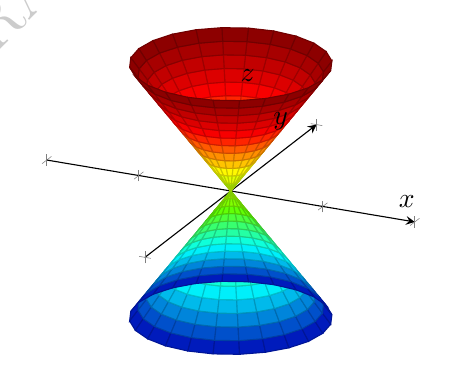
\begin{tikzpicture}
\begin{axis}[colormap/bluered, axis lines=center,
xticklabels={,,}, yticklabels={,,}, zticklabels={,,},
xlabel=$x$, ylabel=$y$, zlabel=$z$,
xmin=-2, xmax=2,
ymin=-2, ymax=2]
\addplot3[surf,domain=-1:1,y domain=0:360,]({x*cos(y)},{x*sin(y)},{x});
\end{axis}
\end{tikzpicture}
\end{minipage}
\begin{minipage}{0.45\textwidth}
\begin{verbatim}
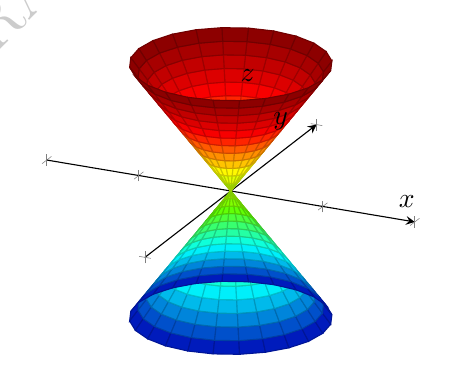
\begin{tikzpicture}
\begin{axis}[colormap/bluered, axis lines=center,
xticklabels={,,}, yticklabels={,,}, zticklabels={,,},
xlabel=$x$, ylabel=$y$, zlabel=$z$,
xmin=-2, xmax=2,
ymin=-2, ymax=2]
\addplot3[surf,domain=-1:1,y domain=0:360,]
    ({x*cos(y)},{x*sin(y)},{x});
\end{axis}
\end{tikzpicture}
\end{verbatim}
\end{minipage}
\subsubsection{Cartesian}
\begin{minipage}{0.45\textwidth}
\centering
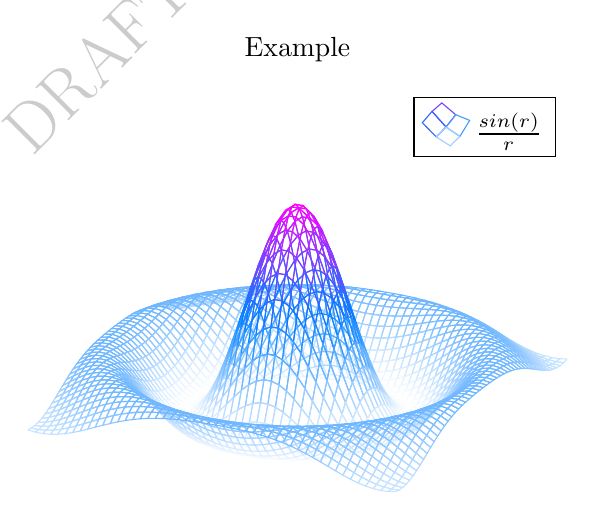
\begin{tikzpicture}
\begin{axis}[colormap/cool, hide axis, title=Example];
\addplot3[mesh,samples=50,domain=-8:8,]{sin(deg(sqrt(x^2+y^2)))/sqrt(x^2+y^2)};
\addlegendentry{$\frac{sin(r)}{r}$}
\end{axis}
\end{tikzpicture}
\end{minipage}
\begin{minipage}{0.45\textwidth}
\begin{verbatim}
\begin{tikzpicture}
\begin{axis}[colormap/cool, hide axis, title=Example];
\addplot3[mesh,samples=50,domain=-8:8,]
    {sin(deg(sqrt(x^2+y^2)))/sqrt(x^2+y^2)};
\addlegendentry{$\frac{sin(r)}{r}$}
\end{axis}
\end{tikzpicture}
\end{verbatim}
\end{minipage}\\
Other color schemes are \verb|hot|, \verb|hot2|, \verb|blackwhite|, \verb|jet|, \verb|bluered|, \verb|cool|, \verb|greenyellow|, \verb|redyellow|, and \verb|violet|.  In three dimensions the default axis type is \verb|box|, other axis options are \verb|left|, \verb|middle|, \verb|center|, \verb|right|, or \verb|none|. 
\appendix
\section{Special Symbols}
\begin{table}[p] \label{table:4}
\renewcommand\arraystretch{1.5}
\setlength\tabcolsep{20pt}
\centering
\begin{tabular}{rl}
\hline
Command & Output\\
\hline
\verb|\today| & \today\\
\verb|\qedsymbol| & \qedsymbol\\
\verb|$mathcal{L}$| & $\mathcal{L}$ \\
\verb|$\vec{v}$| & $\vec{v}$\\
\verb|$\pm \mp$| & $\pm \mp$ \\
\verb|\vdots| & \vdots \\
\verb|$\ddots$| & $\ddots$ \\
\verb|$\cdots$| & $\cdots$ \\
\verb|\ldots| & \ldots \\
\verb|$\iff$| & $\iff$\\
\verb|$\blacksquare$| & $\blacksquare$ \\
\verb|$\stackrel{?}{=}$| & $\stackrel{?}{=}$\\
\verb|$\overbrace{x+y}^\text{real}$| & $\overbrace{x+y}^\text{real}$ \\
\verb|$\underbrace{x-y}_\text{imaginary}$| & $\underbrace{x-y}_\text{imaginary}$\\
\verb|$\xleftarrow[\text{Hey Thomas}]{\text{You're a fruit!}}$| & $\xleftarrow[\text{Hey Thomas}]{\text{You're a fruit!}}$\\
\verb|$\xrightarrow[\text{Hey Thomas}]{\text{You're a fruit!}}$| & $\xrightarrow[\text{Hey Thomas}]{\text{You're a fruit!}}$\\
\hline
\end{tabular}
\caption{Mathematical Symbols}
\end{table}
\printindex
\end{document}